\documentclass{article}

\usepackage{amsfonts}
\usepackage[all]{xy}
\usepackage{amssymb}
\usepackage{amsmath}
\usepackage{mathrsfs}
\usepackage{amsthm}
\usepackage{enumerate}
\usepackage[hidelinks]{hyperref}
\usepackage{ulem}
\usepackage{tikz}  
\usetikzlibrary{arrows.meta}%画箭头用的包
\usepackage{multicol} %用于实现在同一页中实现不同的分栏
\usepackage{geometry}
% \geometry{a4paper,left=1cm,right=1cm,top=1cm,bottom=1cm}

\newtheorem{defn}{Definition}[subsection]
\newtheorem{prop}[defn]{Proposition}
\newtheorem{lem}[defn]{Lemma}
\newtheorem{thm}[defn]{Theorem}
\newtheorem{cor}[defn]{Corollary}
\newtheorem{rmk}[defn]{Remark}
\newtheorem{fact}[defn]{Fact}
\newtheorem{problem}{Problem}
\newtheorem*{ques}{Question}

\setcounter{section}{0}

\title{LSP}
\author{wyz}
\date{\today}

\begin{document}

  % \maketitle
  % \tableofcontents
  % \newpage
\section{Introduction}
The purpose of this article is to show that two different Mori fibre spaces as out put of a klt pair can be linked by composition of  Sarkisov links.

%%%%%%%%%%%%%%%%%%%%%%%%%%%%%%%%%%%%%%%%%%%%%%%%%%%%%%%%%%%%%%%%%%%%%%%%%%%%%%%%%%%%%%%%%%%%%%%%%%%%%%%%%%%%%%%%%%%%%%%%%%%%%%%%%%%%%%%%%%%%%%%%%%%%%%%%%%%%%%%%%%%%%%%%%%%%%%%%%%%%%%%%%%%%%%%%%%%%%%%%%%%%%%%%%%%%%%%%%%%%%%%%%%%%%%%%%%%%%%%%%%%%%%%%%%
%  As an application, we will describe two groups: the group $\operatorname{Cr}_n$ of birational automorphisms of projective space $\mathbb{P}^{n}$ and the group $\operatorname{Aut}\mathbb{A}^{n}$ of automorphisms of affine space $\mathbb{A}^{n}$.  %
%%%%%%%%%%%%%%%%%%%%%%%%%%%%%%%%%%%%%%%%%%%%%%%%%%%%%%%%%%%%%%%%%%%%%%%%%%%%%%%%%%%%%%%%%%%%%%%%%%%%%%%%%%%%%%%%%%%%%%%%%%%%%%%%%%%%%%%%%%%%%%%%%%%%%%%%%%%%%%%%%%%%%%%%%%%%%%%%%%%%%%%%%%%%%%%%%%%%%%%%%%%%%%%%%%%%%%%%%%%%%%%%%%%%%%%%%%%%%%%%%%%%%%%%%%



In this article, varieties means integral schemes over complex number $\mathbb{C}$.
\subsection{Motivation and Main theorem}
% Start with a projective log smooth pair $ \left(X,B\right) $, and assume we can run $ (K_X+B)$-MMP on it. The program may have different results, and the relation of the outputs is defined below:
The \textbf{Minimal model program (MMP)}  aims to classify varieties up to birational equivalent classed, by finding a minimal model all or Mori fibre space. Let $ \left(X,B\right) $ be a (klt) pair, and assume we can run $ (K_X+B)$-MMP on it. Note that the variety appears in the program is called \textbf{result} of the MMP, and the variety where the MMP ends is called the \textbf{output} of the MMP.
\begin{enumerate}
  \item If $\kappa(X,B)\geqslant 0$, then we expected that MMP ends with a \textbf{minimal model}, i.e. a birational map 
    \[
    X \dashrightarrow Y
    \]
    such that $(K_Y+B_Y)$ is nef;
  \item If $\kappa(X,B)= -\infty$, then we expected than MMP ends with a Mori fibre space, i.e. a birational map $X \dashrightarrow Y$ and a surjectiver morphism $Y\to S$ with connected fibres such that $-(K_Y+B_Y)$ is relative ample.
\end{enumerate}
However, for each case the output may not be unique.
\begin{defn}[MMP related]
  Two or more pairs $ \{(X_i,B_i)\} $ are called \textbf{MMP-related} if they are results of $ (K+B) $-MMP over $ \operatorname{Spec}\,\mathbb{C} $ from a nonsingular  projective variety $ W $ and  boundary $ B_W $ with only normal crossing.
\end{defn}

For the first case, we can show that two different minimal model can be linked by flops:
\begin{thm}
  Let $(W,B_W)$ be a $\mathbb{Q}$-factorial terminal pair, and $(X,B),(Y,D)$ are two minimal models of $(W,B_W)$. Then the birational map $X\dashrightarrow Y$ may be factored as sequence of $(K_X+B)$ flops. 
\end{thm}
For the second case, comes our Main theorem:

\begin{thm}
  Let $ f:(X,B)\to S,f':(X',B')\to S' $ be two $ \mathbb{Q} $-factorial log Mori fibre space  with only klt singularities. Suppose they are  MMP-related with an induced  birational map $\Phi$:
  \[ \xymatrix{
    (X,B)\ar[d]_f\ar@{.>}[r]^\Phi&(X',B')\ar[d]^{f'}\\
    S&S'} \]
  Then $ \Phi  $ can be decomposed into sequence of Sarkisov links.
  \end{thm}
\begin{defn}[Sarkisov links]

  The following four types of  birational maps $X\dashrightarrow X_1$ are called Sarkisov links: 
  \[ \xymatrix{
    &Z\ar[ld]_p\ar@{.>}[r]&X_1\ar[dd]^{f_1}\\
    X\ar[d]_f&&\\
    S &&S_1\ar[ll]}\]
  \[ \textbf{I} \]
  \[ \xymatrix{
    &Z\ar[ld]_p\ar@{.>}[r]&Z'\ar[dr]^{q}&\\
    X\ar[d]&&&X_1\ar[d]_{f_1}\\
    S\ar@{=}[rrr]&&&S_1} \]
  \[ \textbf{II} \]
  \[ \xymatrix{
    X\ar[d]_f\ar@{.>}[r]&Z\ar[rd]^{p}&\\
    S\ar[dr]&&X_1\ar[d]^{f_1}\\
    &T&S_1\ar[l]_\sim}\]
  \[ \textbf{III} \]
  \[ \xymatrix{
    X\ar[d]_f\ar@{.>}[rr]&&X_1\ar[d]^{f_1}\\
    S\ar[dr]&&S_1\ar[dl]\\
    &T &}\]
  \[ \textbf{IV} \]
  Here, all $ f:(X,B)\to S $ and $ f_1:(X_1,B_1)\to S_1 $ are log Mori fibre space, and all $ p,q $ are divisorial contractions, and all dash arrows are composition of flips. 
\end{defn}
  An easy example of Mori fibre space is the projecive space $\mathbb{P}^{n}\to pt$. Let $\Phi : \mathbb{P}^{n}\dashrightarrow \mathbb{P}^{n}$ be a birational automorphism, and take a common resolution
  \[
    \xymatrix{
      &W \ar[ld]\ar[rd]&&\\
      \mathbb{P}^{n}\ar[d]& &\mathbb{P}^{n}\ar[d]\\
      pt &&pt
    }
  \]
  then they are MMP-related, and hence can be decomposed into Sarkisov links by the main theorem. In particular, let $\Phi :\mathbb{A}^{n}to \mathbb{A}^{n}$ be an automorphism, then it can be extended into a birational map of $\mathbb{P}^{n}$. Furthermore, one can take $X=X'=\mathbb{P}^{n}$ and $B=B'=\mathbb{P}^{1}$ such that $\Phi: \mathbb{A}^{n}=X\setminus B\to \mathbb{A}^{n}=X'\setminus B'$ is the automorphism. The composition of Sarkisov links helps understanding the groups $\operatorname{Cr}_n$ and $\operatorname{Aut}_n$:
 %%%%%%%%%%%%%%%%%%%%%%%%%%%%%%%%%%%%%%%%%%%%%%%%%%%%
 %  Here we need some corollaries about the groups  %
 %%%%%%%%%%%%%%%%%%%%%%%%%%%%%%%%%%%%%%%%%%%%%%%%%%%%
  
\subsection{Sektch of the proof}
Let $(W,B_W)$ be a log smooth (klt) pair and the MMP ends with a log Mori fibre space $ W\overset{\pi}{\dashrightarrow}(X,B)\xrightarrow{f} S$. Replace $W$ by further resolution and we may assume $\pi$ is a morphism. Take a very general ample divisor $A$ on $S$ and a sufficiently divisible integer $\mu$ such that 
\[
  \mathcal{H}_X=|-\mu(K_X+B)+f^*A|
\]
is a (very) ample linear system on $X$. Furthermore , one can take a general member $H_X\in \mathcal{H}_X $ and a divisor $H_W$ on $W$ such that $\pi_*H_X=H_W=\pi^{-1}_*H_{X}$. Then $(K_X+B+\frac{1}{\mu}H)=\frac{1}{\mu}f^*A$ is nef, therefore $(X,B+\frac{1}{\mu})$ is a minimal model of $(W,B_W+\frac{1}{\mu}H_W)$, and $S$ is the ample model. This marks the position of $X$ with respect to $W$.

The algorithm of decomposing the birational map $\Phi$
\[
  \xymatrix{
    X_{0}=X\ar[d]\ar@{-->}[r]^\Phi &\ar[d] X'\ar[d] \\
    S& S'
  }
\]
is to construct each link 
\[
  \xymatrix{
    X_{0}\ar[d]\ar@{-->}[r] &\ar[d] X_{1}\ar[d] \\
  S_{0}& S_{1}'}
\]
inductivly such that $X_{1}$ is closer to $X'$ than $X_{0}$. There are three methods to decompose $\Phi$.
\subsubsection{Original Method}
The Original proof is firstly given by \textbf{Corti}, works for terminal threfolds, and latter generalized by \textbf{Bruno}, works for klt threfolds. works for terminal threfolds. As the development of MMP and BAB, this method woks for all klt pairs.

The strategy to decompose $\Phi$ is to set up a triple $(\mu,\lambda,e)$ called Sarkisov degree, such that it decreases after decomposing Sarkisov links. First we fix an ample divisor $A'$ on $S'$ and $\mu'$ such that $H'=H_{X'}=-\mu'(K_{X'}+B')+f'^*A'$ is very ample. To construct the link $X_i\dashrightarrow X_{i+1}$ from $X_i\dashrightarrow X'$, we take the common resolution $W_i$, which gives the position of $X'$ with respect to $W_i$. Then we define the triple $(\mu_i,\lambda_i,e_i)$ and construct next link. We need to show that Sarkisov degree goes down for finite times, i.e. after finitely many links, $X_n\to X' $ is an isomorphism.
\subsubsection{Double Scaling}
This proof is given by Hacon, and is generalized by Liu jihao for generalized pairs.

Different from original proof, we start with fixing the common resolution $(W,B_W)$ and mark the position for both Mori fibre space, that is, fix ample $\mathbb{Q}$-divisors $A$ on $S$ and $A'$ on $S'$, such that $G=-(K_X+B)+f^*A$ on $X$ and $H=-(K_{X'}+B')+f'^*A'$ on $X'$ are ample $\mathbb{Q}$-divisors. Furthermore, there are divisors $G_W$ and $H_W$ on $W$ such that $X$ and $X'$ are minimal models of $W$ with respect to $(K_W+B_W+G_W)$ and $(K_W+B_W+H_W)$ and $S$ and $S'$ are ample models. We will find Mori fibre spaces $(X_i,B_i)\to S_i$ such that $(X_i,B_i+g_iG_i+h_iH_i)$ is a minimal model of $(W,B_W+g_iG_W+h_iH_W)$ where

\[
  \begin{aligned}
    1&=h_0\geqslant h_1 \geqslant \cdots \geqslant h_n&=0\\
    0&=g_0\leqslant g_1 \leqslant \cdots \leqslant g_n&=1\\
  \end{aligned}
\]
Furthermore, the birational maps $X_{i}\dashrightarrow X_{i+1}$ are Sarkisov links.
\subsubsection{Ample models}
Similar with second proof, we start with the common resolution $W$. However, instead of marking position of $X$ and $X'$, we will find an affine space $V$ of $\operatorname{Div}_\mathbb{R}(W)$ and an ample divisor $A$ such that 
\begin{itemize}
  \item For any divisor $D$ in
    \[
      D \in \mathcal{E}_A(V)= \{A+\Delta: \Delta \in W \text{and } (K_W+\Delta )\text{ is pseudo-effecive and log canonical }\}
    \]
  there is an ample model of $K_W+D$;
  \item There is a finite partition of $\mathcal{E}_A(V)$, each subset is a polytope and corresponds to an ample model;
  \item One can read off which ample model admits a contraction to another ample model from the combinatorics of the polytopes. In fact, there are maps between two connecting subset.
\end{itemize}
We shall show that each vertice of $\mathcal{E}_A( V )$ gives a sarkisov link, and $\Phi:X\dashrightarrow X'$ is composition of such links.
\section{Original Proof}
In this section, we will prove the Main theorem through the original idea. This is firstly given by Corti for terminal threfolds, and is generalized by Mori for klt threfolds. Due to 

Let $f:(X,B)\to S$ and $f':(X',B')\to S'$ be two MMP-related Mori fibre space, such that they are outputs of $(K_{W}+B_{W})$-MMP on a klt pair $(W,B_W)$,  and let $\Phi:X\to X'$ be the birational map.

\subsection{Prepare}
Suppose $\Phi$ is composition of sarkisov links, then obviously that all $X_i$ and $Z_i$ are birational to $X,X'$ and $W$. In fact we can embed these varieties into a smaller collection of varieties. We started with the MMP related condition:
\begin{lem}
  Let $ \{(X_l,B_l)\} $ be a finite family of $ \mathbb{Q} $-factorial klt pairs, then TFAE:
  \begin{enumerate}[(a)]
    \item They are MMP-related;
    \item There is a nonsingular pair $ (W,B_W) $ with snc boundary, and projective birational morphisms $ f_l:W\to  X_l $ dominating each $ X_l $, such that $ f_{l*}B_W=B_l $ and
      \[ K_W+B_W=f_l^*(K_{X_l}+B_l)+\sum_{exceptional}{a_{li}E_{li}} \]
      with $ a_{li}>0 $ for all $ f_i $-exceptional divisors;
    \item For any two pairs $ (X,B=\sum_ib_iB_i),(X',B'=\sum _jb_j'B_j') $ in the family,  $ a(B_i;X',B')\geqslant -b_i $ and strict inequality holds if and only if $ B_i $ exceptional over $ X' $, and $ a(B'_j;X,B)\geqslant -b'_j $ and strict inequality holds if and only if $ B'_j $ exceptional over $ X $
  \end{enumerate}
\end{lem}
Let $ K=K(X) $ be the function field, and let $ \Sigma=\{\nu\} $ be the set of discrete valutions. 
\begin{defn}
  Fix a function 
  \[ \theta:\Sigma\to [0,1)_\mathbb{Q} \]
  Then we can construct a collection $ \mathcal{C}_\theta $ of pairs  associated to $ \theta $, consists of klt pairs $ (X,B=\sum a_iB_i) $ satisfying
  \begin{enumerate}
    \item $ a_i=\theta(B_i) $;
    \item $ a(E;X,B)>-\theta(E) $ for all $ E $ exceptional over $ X $.
  \end{enumerate} 
\end{defn}
For example, if we take $\theta \equiv 0$ constant, the $\mathcal{C}_{\theta}$ is the collection of all terminal varieties $Y$ birational to $X$. In particular, for our problem we can take a category as following:
\begin{prop}\label{cat}
  Let $ f:(X,B)\to S,f':(X',B')\to S' $ be two $ \mathbb{Q} $-factorial log Mori fibre space  with only klt singularities and MMP-related, inducing a birational map:
  \[ \xymatrix{
      (X,B)\ar[d]_f\ar@{.>}[r]^\phi&(X',B')\ar[d]^{f'}\\
 S&S'} \]
  Suppose  $ B=\sum_ib_iB_i+\sum_jd_jD_j $ and $ B'=\sum_jd_j'D_j+\sum_kb_k'B_k' $, where $ B_i $ are divisors on $ X $ but not on $ X' $, $ B_k' $ are divisors on $ X' $ but not on $ X $, and $ D_j $ are divisors on both $ X $ and $ X' $. By lamma above, $ d_j=d_j' $. Take a rational number $ \epsilon=1-\delta $ such that $ 0<b_i,d_j,b_k', -\operatorname{discrep}(X,B),-\operatorname{discrep}(X',B')<\epsilon<1 $, and fix the function $ \theta:\{\nu\}\to [0,1)_\mathbb{Q} $ as following:
  \begin{itemize}
    \item $ \theta(B_i)=b_i, \theta(D_j)=d_j,\theta(B_k')=b_k'$;
    \item $ \theta(E)=\epsilon $ if $ E $ is exceptional on both $ X $ and $ X' $;
    \item $ \theta(D)=0 $ if $ D $ is a divisor on both $ X $ and $ X' $, but not a component of $ B $ or $ B' $.
  \end{itemize}
  Then the collection $ \mathcal{C}_\theta $ satisfies
  \begin{enumerate}[1)]
    \item $ (X,B) $ and $ (X',B') $ belongs to $ \mathcal{C}_\theta $;
    \item For any finitely many klt pairs $ \{(X_l,B_l)\} $ in $ \mathcal{C}_\theta $, there is an object $ (Z,B_Z)\in \mathcal{C}_\theta $ and projective birational morphisms $ Z\to X_l $ dominating each  $ X_l $ as a process of $ (K+B) $-MMP over $ X_l $ (thus over $ \mathrm{Spec}\,\mathbb{C} $);
    \item Any $ (K+B) $-MMP starting from an object in $ \mathcal{C}_\theta $ stays inside $ \mathcal{C}_\theta $, and so does any $ (K+B+cH) $-MMP where $ H $ is base point free and $ c\in \mathbb{Q}_{>0} $. 
  \end{enumerate}
\end{prop}
Fixing a collection $ \mathcal{C}_\theta $ as in \ref{cat}, then as claimed, we shall define the Sarkisov degree. Suppose $ \Phi $ is defined on $ U\subset X $, then $ \mathrm{codim}\,(X-U,X)\geqslant 2 $ since $ X $ is normal. If we fix a very ample divisor $ A'  $ on $ S' $ and a sufficiently large and divisible integer $ \mu'>1 $ such that 
\[ \mathcal{H}'=|-\mu' (K_{X'}+B') +f'^*A'| \]
is a very ample complete linear system on $ X' $ over $ \mathrm{Spec}\,\mathbb{C} $,  inducing an embedding into $ \mathbb{P}^N $ for some $ N $. Pull back $ (\Phi|_U)^*\mathcal{H}' $ of the linear system is a base point free linear system on $ U $, and can be extended  to a movable linear system on $ X $, which coincides with strict transform $ \mathcal{H}:=\Phi^{-1}_*\mathcal{H}' $ , and induces a rational map $ X\dashrightarrow \mathbb{P}^N $. Let $ (W,B_W) $ be a common log resolution of $ X $ and $ X' $ in $ \mathcal{C}_\theta $ with projective birational morphism $ \sigma:W\to X$,   $\sigma':W\to X' $ and $\sigma_*B_W=B, \sigma'_*B_W=B' $, denote
\[ \mathcal{H}_W:=\sigma'^*\mathcal{H}' \]
and then 
\[ \mathcal{H}:=\Phi^{-1}_*\mathcal{H}'=\sigma_*\mathcal{H}_W \]
Furthermore, if $ \mathcal{H} $ is not base point free, then
\[ \sigma^*\mathcal{H}=\mathcal{H}_W+F \]
where $ \sum f_lF_l=F\geqslant0 $ is the fixed part, and $ \sigma(\mathrm{Supp}\,F)\subset X-U $. 

Take a general member $ H' $ of the linear system $ \mathcal{H}' $ such that $ H_W:=\sigma'^*H'=\sigma'^{-1}_*H'\in \mathcal{H}_W $, and let $ H:=\Phi^{-1}_*H'=\sigma_*H $, then $ \sigma^*H=H_W+F $. Since $ \rho(X/S)=1 $ (($\rho( X'/S')=1 $), any effective divisor on $ X $ ($ X' $) is $ f $($ f' $)-ample, including $ H $($ H' $). Now we can define the Sarkisov degree:
\begin{defn}[Sarkisovdegree]
  Sarkisov degree of $ (X,B) $ with respect to $ H $ ($ \mathcal{H} $) in $ \mathcal{C}_\theta $ is a triple $ (\mu,\lambda,e) $ ordered lexicographically:
  \begin{itemize}
    \item Nef threshold $ \mu $: Let $ C\subset X  $ be a curve contracted by $ f $, then 
      \[ \mu:=-\frac{H.C}{(K_X+B).C} \]
      i.e. $ K_X+B+\frac{1}{\mu} H \equiv_S0$ and hence $ f^*A=K_X+B+\frac{1}{\mu} H $ for some $ \mathbb{Q} $-divisor on $ S $;
    \item $ \theta $-canonical threshold $ \lambda $: Take a common log resolution  $ (W,B_W)\in \mathcal{C}_\theta $ with $ B_W=\sum \theta(E)E $ and projective birational morphisms $ \sigma:W\to X $, $ \sigma':W\to X' $. Take a general member $ H'\in \mathcal{H}' $ such that $ H_W:=\sigma'^{-1}_*H'=g^{-1}_*H $. Suppose $ \sigma^*H=H_W+\sum f_lF_l $ with $ \sum f_lF_l $ effective and $ \sigma $-exceptional (by negativity lemma), then we have ramification formulas
      \[ K_W+B_W=\sigma^*(K_X+B+cH)+\sum a_lE_l  \]
      \[ K_W+B_W+cH_W=\sigma^*(K_X+B+cH)+\sum(a_l-cf_l)E_l \]
      where $ \sum a_lE_l $ is effective and supported on $ \mathrm{Exc}\,\sigma $.   Let
      \[ \lambda:=\max\{ \frac{f_l}{a_l}\} \]
      This is independent on the choice of log resolution. In fact $ \frac{1}{\lambda} $ is called $ \theta $-canonical threshold with respect to $ (X,B;H) $, i.e.
      \[ \frac{1}{\lambda}:=\max\{c:a(E;X,B+cH)\geqslant-\theta(E) ,E\text{ exceptionl over }X \}\] 
      If $ \mathcal{H} $ is base point free, then $ \sum f_lF_l=0 $ and $\sum(a_l-cf_l)E_l\geqslant 0  $ always holds, in which case $ \lambda=0 $ by definition;
    \item $ e=0 $ if $ \mathcal{H} $ is base point free (and hence $ \lambda=0 $), otherwise 
      \[ e=\#\{E_i; E_i \text{ is }\sigma\text{-exceptional and } a(E;X,B+\frac{1}{\lambda} H)=-\theta(E) \} \]
      or equivalently in the formular 
      \[ K_W+B_W+\frac{1}{\lambda} H_W=\sigma^*(K_X+B+\frac{1}{\lambda} H)+\sum(a_l-cf_l)E_l \]
      $ e $ is the number of components in $ E-\frac{1}{\lambda} F $ with coefficient $ 0 $. 
  \end{itemize}
\end{defn}
In particular, if $\Phi:X\to X'$ is already an isomorphism, then $\mu=\mu'$ and $\lambda=e=0$; conversely, we have the Noether-Fano-Iskovskikh criterion to show when they are isomorphic:
\begin{thm}\label{nfi}
  (Noether-Fano-Iskovskikh Criterion): Notations as in the definition of Sarkisov degree, then 
  \begin{enumerate}
    \item $ \mu\geqslant \mu' $;
    \item If $ \mu \geqslant \lambda $ and $ (K_X+B+\frac{1}{\mu} H) $ is nef, then we have an isomorphism
      \[ \xymatrix{
          X\ar[r]^\sim_\Phi\ar[d]_f&X'\ar[d]^{f'}\\
      S\ar[r]^\sim& S' } \]
  \end{enumerate}
\end{thm}
To proof the criterion \ref{nfi}, we need following lemmas
\begin{lem}\label{extraction}
Let $ (X,B) $ be a a klt pair and $\Sigma$ be any set of exceptional divisors such that  contains only exceptional divisors $ E $ of dicrepancy $ a(E;X,B)\leqslant 0 $. Then there is a birational morphism $ f:Z\to X $ and a $ \mathbb{Q} $-divisor $ B_Z $such that:
  \begin{enumerate}
    \item $ (Z,B_Z) $ is klt;
    \item $ E $ is an exceptional divisor for $ f $ if and only if $ E\in\Sigma $;
    \item $ B_Z=\sum-a(E;X,B) $ and $ f_*B_Z=B $ and $ K_Z+B_Z=f^*(K_X+B) $.
  \end{enumerate} 
  In particular, if we take $ \Sigma $ containing all such divisors, then $ Z $ is called \textbf{terminalization} of $ X $; if take $ \Sigma $ containing only one such divisor, then $ f:Z\to X $ is called a \textbf{divisorial extraction}.    
\end{lem}

For our case,
\begin{lem}[maximal crepant blow up]
Let $ (X,B) $ be a $ \mathbb{Q} $-factorial $ \theta $-terminal pair and $ (X,B+H) $ is $ \theta $-canonical where $ H$ is a effective divisor. A \textbf{maximal crepant blow up} is a projective birational morphism $ p:(Z,B_Z)\to (X,B) $ from a $ \theta $-terminal pair in $ \mathcal{C}_\theta $ such that
  \begin{enumerate}
    \item $ p_*B_Z=B $;
    \item $ K_Z+B_Z+p^{-1}_*H=p^*(K_X+B+H) $;
    \item $ (Z,B_Z+p^{-1}_*H) $ is a $ \mathbb{Q} $-factorial $\theta $-terminal pair.
  \end{enumerate}  
\end{lem}

\begin{proof}[proof of \ref{nfi}]
  \begin{enumerate}
    \item Only need to show $ (K_X+B+\frac{1}{\mu'}H) $ is $ f $-nef. Notations as above, we have
      \[ \xymatrix{
      &(V,B_V,H_V)\ar[dl]_g\ar[dr]^{g'}&\\
          (X,B,H)\ar[d]_f\ar@{.>}[rr]^\Phi&&(X',B',H')\ar[d]^{f'}\\
      S&&S'} \]
      Consider the ramification formulas:
      \[
        \begin{aligned}  
          K_V+B_V+\frac{1}{\mu'}H_V=&g'^*(K_{X'}+B'+\frac{1}{\mu'}H')+\sum e'_jE_j+ \sum g_k'G_k'\\
          =&g^*(K_{X}+B+\frac{1}{\mu'}H)+\sum g_iG_i+\sum e_jE_j
        \end{aligned}
      \]
      Here $ \{G_i\}, \{E_j\} $ are $ g $-exceptional divisors, and $ \{E_j\}\{G'_k\} $ are $ g' $-exceptional divisors. Since $H_V:=g'^*H' $, $ g_k'>0 $ (or there are no such $ G'_k $). Then take a general curve $ C\subset X $ contracted by $ f $,  avoiding $ G_i, E_j $, and not contained in $ G'_k $, and identifies its strict transform $ \tilde{C} $ in $ V $ with $ C $. By computing intersection numbers:
      \[
        \begin{aligned}
          C.(K_X+B+\frac{1}{\mu'}H)=&\tilde{C}.g^*(K_X+B+\frac{1}{\mu'}H)
          \\=&C.((K_X+B+\frac{1}{\mu'}H)+\sum g_iG_i+\sum e_jE_j)\\
          =&C.(K_V+B_V+\frac{1}{\mu'}H_V)\\
          =&C.(g'^*(K_{X'}+B'+\frac{1}{\mu'}H')+\sum e'_jE_j+ \sum g_k'G_k')\\
          =&C.g'^*f'^*A'+C.(\sum g_k'G_k')\\
          \geqslant&0
        \end{aligned}
      \]
      Since $ A' $ is ample on $ S' $, and $ g'_k>0 $. This shows $ (K_X+B+\frac{1}{\mu'}H) $ is $ f $-nef and $ \mu\geqslant \mu' $;
    \item We prove this in 4 steps.

      \textbf{Step1}: $ \mu=\mu' $

      By 1), dually only need to show $ (K_{X'}+B'+\frac{1}{\mu}H') $ is $ f' $-nef. Take a curve $ C' $ similar as above, then
      \[
        \begin{aligned}
          C'.(K_{X'}+B'+\frac{1}{\mu}H')=&C'.(g^*(K_{X}+B+\frac{1}{\mu}H)+\sum e_jE_j+ \sum g_k'G'_k)\\
          =&C'.(g^*(K_{X}+B+\frac{1}{\mu}H)+C.(\sum g_k'G_k')\\
          \geqslant&0
        \end{aligned}
      \]
      Since $ K_{X}+B+\frac{1}{\mu}H $ is nef , $ C' $ not contained in $ G'_k $, and $ g_k'\geqslant 0 $ by $ \lambda\leqslant \mu. $

      \textbf{Step2}: In the ramification formular above, $ g_i=0, e_i=e_i' $ and $ \{G'_k\}=\emptyset $.

      Since $ \mu=\mu' $, equations (1) shows
      \[ \sum(e_j-e'_j)+\sum g_iG_i\equiv_X g'^*f'^*A'+\sum g_k'G'_k \]
      \[ \sum(e'_j-e_j)+\sum g_k'G'_k\equiv_{X'} g^*(K_{X}+B+\frac{1}{\mu}H)+\sum g_iG_i \]
      By negativity lemma, $ (e_j-e'_j), (e'_j-e_j), g_i,g_k'\leqslant 0$. By choice of $ (V,B_V) $, we have $ e'_i,g'_k>0 $; and since $\lambda\leqslant\mu$, we have $ g_i\geqslant 0 $. These implies step 2, and 
      \[ g^*(K_{X}+B+\frac{1}{\mu}H)=g'^*(K_{X'}+B'+\frac{1}{\mu}H') \]

      Furthermore, any curve $ C\subset V $ contracted by $ fg $, we have
      \[
        \begin{aligned}
          0=&C.g^*(K_{X}+B+\frac{1}{\mu}H)\\
          =&C.g'^*(K_{X'}+B'+\frac{1}{\mu}H') \\
          =&C.g'^*f'^*A'
        \end{aligned}
      \]
      Since $ A' $ is ample on $ S' $, $ C $ is contracted by $ f'g' $. By Rigidity lemma, there is a morphism $ \tau:S\to S' $.

      \textbf{Step3}: $ \Phi $ is isomorphic in codimension 1, and conclude the result.

      Notice that $ \{G_i\} \{E_j\} $ are $ g $-exceptional and $ \{E_j\} $ are $ g' $-exceptional, only need to show there is no $ G_i $. Take the extraction $ p:(Z,B_Z,\frac{2}{\mu} H_Z)\to (X,B,\frac{1}{\mu} H) $ by \ref{extraction} for all $\{E_{i}\} $, then $ G_i $ are exactly divisors on $ Z $ exceptional over $ X $, thus $ Z,V,X' $ are isomorphic in codimension $ 1 $. Take a very ample divisor $ D_Z $ on $ Z $ and let $ D'  $ be strict transform on $ X' $, $ D' $ is $ f' $-ample since it is effective and $ \rho(X'/S')=1 $ , thus for some $ 0<d\ll1 $ 
      \begin{itemize}
        \item $ K_Z+B_Z+\frac{1}{\mu }H_Z+dD_Z $ is ample since $ K_Z+B_Z+\frac{1}{\mu }H_Z=p^*(K_X+B+\frac{1}{\mu }H) $ is nef;
        \item $ K_{X'}+B'+\frac{1}{\mu }H'+dD' $ is ample since $ K_{X'}+B'+\frac{1}{\mu }H' $ is pull back of ample divisor $ \frac{1}{\mu'}A' $ on $ S' $ and $ D' $ is $ f' $-ample.
      \end{itemize}
      Therefore $ X' $ isomorphic to $ Z $.
      \[ \xymatrix{
          Z\ar[r]^\sim\ar[d]_p&X'\ar[dd]^{f'}\\
          X\ar[d]_f\ar@{.>}[ur]^\Phi&\\
      S\ar[r]^\tau&S' } \]
      Picard number also shows $ \rho(Z/X)=0 $ and $ X\xrightarrow[\Phi]{\sim}X' $.
  \end{enumerate}
\end{proof}

\subsection{Construct Sarkisov links inductively}\label{constructlink1}
In this section, we construct the links inductively. If $ \lambda\leqslant\mu $ and $ K_X+B+\frac{1}{\mu}H $ is nef, then by Noether-Fano-Iskovskikh Criterion \ref{nfi}, $ \Phi $ is an isomorphism and we stop here.
\begin{enumerate}[(A)]
  \item\label{1A} If $ \lambda\leqslant\mu $ and $ K_X+B+\frac{1}{\mu}H $ is not nef, suppose $ f $ is the contraction with respect to a $ (K_X+B) $-negative extremal ray $ R= \overline{\operatorname{ NE }}(X/S) $, then $ (K_X+B+\frac{1}{\mu}H).R=0 $ by definition of $ \mu $. \textbf{Claim} that there is an extremal ray $ P\in \overline{\operatorname{ NE }}(X) $ such that $ (K_X+B+\frac{1}{\mu}H).P<0 $ and $ F:=P+R $ is an extremal face.
    \begin{proof}[proof of the claim]
    ( Corti, Factoring birational maps of 3-fold after Sarkisov ) Surjective map $ f_*:N_1(X)\to N_1(S) $ can be identified with $ \pi: N_1(X)\to N_1(X)/\pm R $ and $ \pi(\overline{\operatorname{NE}}(X))=\overline{\operatorname{NE}}(S) $. Since $ (K_X+B+\frac{1}{\mu}H) $ is trivial on $ R $ and not nef, it is pull back $ f^*A $ of a non nef divisor $ A $ on $ S $. By the cone theorem of $ (B+\frac{1}{\mu}H) $, $ \overline{\operatorname{NE}}(X)_{A<0} $ is a locally finitely generated polyhedral, thus there is an  $ A $-negative extremal ray $ \hat{P}=D^\perp\cap \overline{\operatorname{NE}}(S) $ where $ D $ is a nef divisor on $ S $. Now consider the extremal face $ F $ with respect to$ f^*D $ ($ F=\pi^{-1}(\pm \hat{P})\cap \overline{\operatorname{NE}}(X) $), clearly $ F=R+P $ where $ P $ is the lift ray of $ \hat P $. Furthermore, $ (K_X+B+\frac{1}{\mu}H).P=A.\hat P<0 $.
\end{proof}
  Take  $ 0<t\ll 1 $ such that $ (K_X+B+(\frac{1}{\mu}-t)H).P<0 $, then $  (K_X+B+(\frac{1}{\mu}-t)H).R<0 $ and $ F $ is a $  (K_X+B+(\frac{1}{\mu}-t)H) $-negative extremal face. Since $ (X,B+(\frac{1}{\mu}-t)H) $ is klt, there is  a contraction $ g:X\to T $ with respect to to $ F $ factorizing through $ f:X\to S $: 
  \[ \xymatrix{
    X\ar[d]_f\ar[ddr]^g&\\
    S\ar[dr]&\\
    &T }\]
  $ (X,B+\frac{1}{\mu}H) $ is klt, and $ \rho(X/T)=2 $, thus we can  run $ (K_X+B+\frac{1}{\mu}H) $-MMP on $ X $ over $ T $ as a 2-ray game: Identify $ \overline{\operatorname{NE}}(X/T) $ with $ F=R+P $, since $ (K_X+B+\frac{1}{\mu}H).P<0 $, there is a contraction with respect to $ P $ over $ T $. If the contraction is a flip
  \[ \xymatrix{
    X\ar[ddr]_g\ar@{.>}[rr]\ar[rd]^h&&X^+\ar[ddl]^{g^+}\ar[ld]_{h^+}\\
    &Y\ar[d]&\\
    &T&} \] 
  then $ (K_{X^+}+B^++\frac{1}{\mu}H^+) $ is $ g^+ $-ample, and $ \rho(X^+/T)=2 $, and isomrophic in codimension 1. $ (X^+,B^++\frac{1}{\mu}H^+)/T $ is a minimal model, or there is a negative extremal ray and MMP goes on. The sequence of flips is finite, and the first non-flip contraction is either a divisorial contraction or a fibering contraction.
  
  By BCHM, $ B+\frac{1}{\mu}H $ is relatively big, thus the MMP terminates with one of following results: 
  \begin{enumerate}[1)]
    \item If after finitely many flips $ X\dashrightarrow Z $, first non-flip contraction is a divisorial contraction $ p:Z\to X_1\xrightarrow{g_1}T $, and the MMP ended with a Mori fibre space.  Since $ \rho(X_1/T)=1 $, there is no further flips or divisorial contraction, thus must be followed by a fibering contraction $ f_1:X_1\to Y $ with $ Y\xrightarrow{\sim}T $.
    \[ \xymatrix{
      X\ar[d]_f\ar[ddr]^g\ar@{.>}[r]^{flips}&Z\ar[rd]^{p}&\\
      S\ar[dr]&&X_1\ar[d]^{f_1}\ar[ld]_{g_1}\\
      &T&Y\ar[l]_\sim}\]
    Furthermore, we can take $ H' $ general enough (avoid the divisor contracted by $ p $) such that $ H_1 $ is strict transform of $ H $ and $ H' $. Since $ \rho(X_1/Y)=1 $ and $ H_1 $ is effective, $ H_1 $ is $ f_1 $-ample, thus $ (K_{X_1}+B_1) $ is $ f_1 $-negative and $ (X_1,B_1)/Y $ is a log Mori fibre space.  Take $ S_1=Y $.
    \[ \xymatrix{
      X\ar[d]_f\ar@{.>}[r]^{flips}&Z\ar[rd]^{p}&\\
      S\ar[dr]&&X_1\ar[d]^{f_1}\\
      &T&S_1\ar[l]_\sim}\]
    This is a link of type III.     
    \item If after finitely many flips $ X\dashrightarrow X_1 $, first non-flip contraction is a fibering contraction $ f_1:X_1\to Y  $
    \[ \xymatrix{
      X\ar[d]_f\ar[ddr]^g\ar@{.>}[rr]^{\psi_1}&&X_1\ar[d]^{f_1}\ar[ddl]_{g_1}\\
      S\ar[dr]&&Y\ar[dl]\\
      &T &}\]
    Same as above, $ (X_1,B_1)/Y $ is a log Mori fibre space. Take $ S_1=Y $
    \[ \xymatrix{
      X\ar[d]_f\ar@{.>}[rr]^{\psi_1}&&X_1\ar[d]^{f_1}\\
      S\ar[dr]&&S_1\ar[dl]\\
      &T &}\]
    this is a link of type IV. 
    \item If after finitely many flips $ X\dashrightarrow Z $, first non-flip contraction is a divisorial contraction $ p:Z\to X_1\xrightarrow{g_1}T $ with 
    \[ K_Z+B_Z+\frac{1}{\mu}H_Z=p^*(K_{X_1}+B_1+\frac{1}{\mu}H_1)+eE \]
    where $ e>0 $ and the MMP ended with a log minimal model. Since  $ \rho(X_1/T)=1 $, $ (X_1,B_1+\frac{1}{\mu}H_1) $ must be the log minimal model.
    \[ \xymatrix{
      X\ar[d]_f\ar[ddr]^g\ar@{.>}[r]^{flips}&Z\ar[rd]^{p}&\\
      S\ar[dr]&&X_1\ar[dl]_{g_1}\\
      &T&}\]
    Claim that the only ray of $ \overline{\operatorname{NE}}(X_1/T) $ is $ (K_{X_1}+B_1+\frac{1}{\mu}H_1) $-trivial. Indeed, take a curve $ C_1\subset X_1 $ contracted by $ g_1 $ away from indeterminacy of $ X_1\dashrightarrow X $ ( union of image of exceptional divisor of $ p $ and all flipped curves) and not contained in the base locus of $ \mathcal{H}_1 $, then $ C $ can be considered also to lie on $ X $ and contracted by $ g $ and $ H_1.C\geqslant 0 $.  The union of  indeterminacy locus and base locus of $ \mathcal{H}_1 $ is a closed subset of $ X_1 $, thus suppose there is an open subset $ U_1 $ of $ X_1 $ avoiding that closed subset, and  isomorphic to an open subset $ U $ of $ X $. Then  thus $ [C]\in F $ and
    \[
      \begin{aligned}
        0\geqslant& (K_X+B+\frac{1}{\mu}H).C_X\\
        =&(K_Z+B_Z+\frac{1}{\mu}H_Z).C_Z\\
        \geqslant&(K_Z+B_Z+\frac{1}{\mu}H_Z-eE).C\\
        =&(K_{X_1}+B_1+\frac{1}{\mu}H_1).C\geqslant 0\\
      \end{aligned}
    \]
    Therefore $ (K_{X_1}+B_1+\frac{1}{\mu}H_1).C_1=0 $. Furthermore, $ H_1 $ is effective, thus is $ g_1 $-ample, and hence $ (K_{X_1}+B_1) $ is $ g_1 $-negative, and $ (X_1,B_1)/T $ is a log Mori fibre space. Take $ S_1=T $
    \[ \xymatrix{
      X\ar[d]_f\ar@{.>}[r]&Z\ar[rd]^{p}&\\
      S\ar[dr]&&X_1\ar[d]^{f_1}\\
      &T&S_1\ar@{=}[l]}\]
    This is a link of type III. Since $ (K_{X_1}+B_1+\frac{1}{\mu}H_1) $ is trivial on the ray $ R=\overline{\operatorname{NE}}(X_1/S_1) $, we  have 
    \[ \mu=\mu_1 \]
    Notice that $ (X_1,B_1+\frac{1}{\mu}H_1) $ stays $ \theta $-canonical, we have
    \[ \lambda_1\leqslant \mu=\mu_1 \]
    Furthermore, $ \rho(X_1)=\rho(X)-1 $.
    \item If after finitely many flips $ X\dashrightarrow X_1 $, MMP ends with log minimal model $ (X_1,B_1+\frac{1}{\mu}H_1)/T $
    \[ \xymatrix{
      X\ar[d]_f\ar[ddr]^g\ar@{.>}[rr]^{flips}&&X_1\ar[ddl]_{g_1}\\
      S\ar[dr]&&\\
      &T &}\]
    Claim that there is a ray of $ \overline{\operatorname{NE}}(X_1/T) $ is $ (K_{X_1}+B_1+\frac{1}{\mu}H_1) $-trivial and $ (K_{X_1}+B_1) $-negative. Indeed, take a curve $ C\subset X_1 $ contracted by $ g_1 $ away from indeterminacy of $ X_1\dashrightarrow X $ ( union of all flipped curves) and not contained in the base locus of $ \mathcal{H}_1 $, then $ C $ can be considered also to lie on $ X $ and contracted by $ g $ and $ H_1.C\geqslant 0 $, thus $ [C]\in F $ and
    \[
      \begin{aligned}
        0\geqslant& (K_X+B+\frac{1}{\mu}H).C\\
        =&(K_{X_1}+B_1+\frac{1}{\mu}H_1).C\geqslant 0\\
        0> &(K_X+B+(\frac{1}{\mu}-t)H).C\\
        =&(K_{X_1}+B_1+(\frac{1}{\mu}-t)H_1).C\geqslant (K_{X_1}+B_1).C
      \end{aligned}
    \]
    Take a contraction $ f_1:X_1\to S_1 $ with respect to $ (K_{X_1}+B_1) $-negative ray $ R=\mathbb{R}_{\geqslant 0}[C] $
    \[ \xymatrix{
      X\ar[d]_f\ar@{.>}[rr]&&X_1\ar[d]^{f_1}\\
      S\ar[dr]&&S_1\ar[dl]\\
      &T &}\]
    This is a link of type IV. Since $ (K_{X_1}+B_1+\frac{1}{\mu}H_1) $ is trivial on the ray $ R=\overline{\operatorname{NE}}(X_1/S_1) $, we  have 
    \[ \mu=\mu_1 \]
    Notice that $ (X_1,B_1+\frac{1}{\mu}H_1) $ stays $ \theta $-canonical, we have
    \[ \lambda_1\leqslant \mu=\mu_1 \]
  \end{enumerate}
  \item If $ \lambda>\mu $, then $ (X,B+\frac{1}{\mu}H) $ is not $ \theta $-canonical. Take a extremal blow up $ p:(Z,B_Z,H_Z)\to (X,B,H) $ in $ \mathcal{C}_\theta $ with respect to $ K_X+B+\frac{1}{\lambda}H $, i.e. $ (Z,B_Z) $ is $ \theta $-terminal and $ p^*(K_X+B+\frac{1}{\lambda}H)=K_Z+B_Z+\frac{1}{\lambda}H_Z $ where $ B_Z=\sum\theta(E_\nu)E_\nu $ and $ E=\mathrm{Exc}\,p $ is a prime divisor on $ Z $.  Let $ H_Z=p^{-1}_*H $ a strict transform of a general member $ H' $ of $ \mathcal{H}' $: 
  \[ \xymatrix{
    &Z\ar[ld]_p\ar[ldd]\\
    X\ar[d]&\\
    S} \]
  Run $ (K_Z+B_Z+\frac{1}{\lambda}H_Z) $-MMP on $ Z $ over $ S $, then it always ends with a Mori fibre space. Otherwise, there are two cases:
  \begin{enumerate}[a)]
    \item After finitely many flips $ Z\dashrightarrow Z' $, first non flip contraction is a divisorial contraction $ q:Z'\to X_1 $. Since $ \rho(X_1/S)=1 $, $ (X_1,B_1+\frac{1}{\lambda}H_1) $ must be the ending log minimal model.
      \[ \xymatrix{
      &Z\ar[ld]_p\ar[rdd]^{g}\ar@{.>}[rr]^{flips}&&Z'\ar[dr]^{q}&\\
      X\ar[drr]\ar@{.>}[rrrr]^{\psi_1}&&&&X_1\ar[dll]^{g_1}\\
      &&S&&} \]
    Let $ E_q=\mathrm{Exc}\,q $ be the exceptional divisor, then 
    \[ K_{Z'}+B_{Z'}+\frac{1}{\lambda}H_{Z'}=q^*(K_{X_1}+B_1+\frac{1}{\lambda}H_1)+aE_q \,(a>0)\]
    Take a curve $ C_X\subset X $ contracted by $ f $ and away from $ p(E) $ (thus can be considered to be a curve $ C_Z $ on $ Z $) and flipped curves (thus can be considered to be a curve $ C_{Z'} $ on $ Z' $) and $ E_q $ (thus $ E_q.C_Z\geqslant 0 $ ), then
    \begin{equation*}
      \begin{aligned}
        0\leqslant& (K_{X_1}+B_1+\frac{1}{\lambda}H_1).q_*C_{Z'} \text{ (it is minimal model)}\\
        =&(K_{Z'}+B_{Z'}+\frac{1}{\lambda}H_1-aE_q).C_{Z'}\\
        =&(K_{Z}+B_{Z}+\frac{1}{\lambda}H_1-aE_q).C_{Z}\\
        \leqslant &(K_{Z}+B_{Z}+\frac{1}{\lambda}H_1).C_{Z}\\
        =&(K_X+B+\frac{1}{\lambda}H).C_X\\
        <&(K_{X}+B+\frac{1}{\mu}H).C_X  \,(\frac{1}{\lambda}<\frac{1}{\mu})\\
        =&0
      \end{aligned}
    \end{equation*} 
  Contraction!
  \item If after finitely many flips $ Z\dashrightarrow X_1 $,  $ (X_1,B_1+\frac{1}{\lambda}H_1) $ is the ending log minimal model.
    \[ \xymatrix{
    &Z\ar[ld]_p\ar[ldd]\ar@{.>}[r]^{flips}&X_1\ar[lldd]^{g_1}\\
    X\ar[d]_f&&\\
    S &&}\]
    Take a curve $ C_X\subset X $ contracted by $ f $ and away from $ p(E) $ (thus can be considered to be a curve $ C_Z $ on $ Z $) and flipped curves (thus can be considered to be a curve $ C_{1} $ on $X_1$). Then
    \begin{equation*}
      \begin{aligned}
        0\leqslant& (K_{X_1}+B_1+\frac{1}{\lambda}H_1).C_1 \text{ (it is minimal model)}\\
        =&(K_{Z}+B_{Z}+\frac{1}{\lambda}H_1).C_{Z}\\
        = &(K_X+B+\frac{1}{\lambda}H).C_X\\
        <&(K_{X}+B+\frac{1}{\mu}H).C_X  \,(\frac{1}{\lambda}<\frac{1}{\mu})\\
        =&0
      \end{aligned}
    \end{equation*} 
  Again  a contradiction!
  \end{enumerate}  
  Thus we may assume the MMP ends with a Mori fibre space:
  \begin{enumerate}[1)]
    \item After finitely many flips $ Z\dashrightarrow Z' $, first non flip contraction is a divisorial contraction $ q:Z'\to X_1 $. Since $ \rho(X_1/S)=1 $, there is no further flips or divisorial contraction, thus must be followed by a fibering contraction $ f_1:X_1\to Y $ with $ Y\xrightarrow{\sim}S $.
    \[ \xymatrix{
      &Z\ar[lddd]^g\ar[ld]_p\ar@{.>}[r]&Z'\ar[dr]^{q}\ar[llddd]^{g'}&\\
      X\ar[dd]&&&X_1\ar[dd]_{f_1}\ar[ddlll]^{g_1}\\
      &&&\\
      S&&&Y\ar[lll]_{\sim}} \]
    Since $ (K_{X_1}+B_1+\frac{1}{\lambda}H_1) $ is $ f_1 $-negative, and $ H_1 $ is $ f_1 $- ample, $ (K_{X_1}+B_1) $ is $ f_1 $-negative, and $ (X_1,B_1)/Y $ is a log Mori fibre space.  Take $ S_1=Y $.
    
    \[ \xymatrix{
      &Z\ar[ld]_p\ar@{.>}[r]&Z'\ar[dr]^{q}&\\
      X\ar[d]\ar@{.>}[rrr]^{\psi_1}&&&X_1\ar[d]_{f_1}\\
      S\ar@{=}[rrr]&&&S_1} \]
    This is a link of type II.
    \item If after finitely many flips $ Z\dashrightarrow X_1 $, first non-flip contraction is a fibering contraction $ f_1:X_1\to Y  $ 
    \[ \xymatrix{
      &Z\ar[ld]_p\ar[ldd]\ar@{.>}[r]^{flips}&X_1\ar[lldd]^{g_1}\ar[dd]^{f_1}\\
      X\ar[d]_f&&\\
      S &&Y\ar[ll]}\]
    Since $ (K_{X_1}+B_1+\frac{1}{\lambda}H_1) $ is $ f_1 $-negative, and $ H_1 $ is $ f_1 $- ample, $ (K_{X_1}+B_1) $ is $ f_1 $-negative, and $ (X_1,B_1)/Y $ is a log Mori fibre space.  Take $ S_1=Y $.
    \[
      \xymatrix{
      &Z\ar[ld]_p\ar@{.>}[r]&X_1\ar[dd]^{f_1}\\
        X\ar[d]_f&&\\
      S &&S_1\ar[ll]}
    \]
    This is a link of type I.
  \end{enumerate} 
\end{enumerate}

In the process of log Sarkisov program, the Sarkisov degree changes as following:
\begin{enumerate}[(A)]
  \item 
  \begin{enumerate}[1)]
    \item For case (A)-1),2),  since $ K_{X_1}+B_1+\frac{1}{\mu}H_1 $ is $ f_1 $-negative, we have 
    \[ \mu_1<\mu \]
    \item For case (A)-3),4), Since $ (K_{X_1}+B_1+\frac{1}{\mu}H_1) $ is trivial on the ray $ R=\overline{\operatorname{NE}}(X_1/S_1) $ for both case, we have
    \[ \mu_1=\mu \]
    Notice that $ (X_1,B_1+\frac{1}{\mu}H_1) $ stays $ \theta $-canonical, we have
    \[ \lambda_1\leqslant \mu=\mu_1 \]
    Thus this go back to case (A). Furthermore,   for case (A)-3) we have
    \[ \rho(X_1)=\rho(X)-1 \]
    and for case (A)-4), the birational map
    \[ X\dashrightarrow X_1 \]
    is composition of finitely many flips.
  \end{enumerate} 
  \item For case (B): 
  \begin{enumerate}[1)]
    \item For both case B-1),2), claim that 
    \[ \mu_1\leqslant \mu \]
    with equality holds if and only if 
    \begin{equation*}
      \begin{aligned}
        \text{either } &\dim S_i<\dim S_{i+1} \\
        \text{or }&\dim S_i=\dim S_{i+1} \text{ and the link is square} 
      \end{aligned}
    \end{equation*} 
    Indeed, since $ \lambda>\mu $, we have a ramification fomular
    \[ K_Z+B_Z+\frac{1}{\mu}H_Z=p^*(K_X+B+\frac{1}{\mu}H)+bE, b>0 \]
    Take a curve $ C_1\subset X_1 $ contracted by $ f_1 $ away from locus of indeterminacy of the birational map $ X_1\dashrightarrow Z $, then $ C_1 $ is also a curve lies on $ Z $, then
    \begin{equation*}
      \begin{aligned}
        0=& (K_{X}+B+\frac{1}{\lambda}H).p_*C \text{ (by definition of )} \mu\\
        =&(K_{Z}+B_{Z}+\frac{1}{\lambda}H_Z+bE).C_{Z}\\
        \geqslant&(K_Z+B_Z+\frac{1}{\lambda}H_Z).C_Z\\
        =&(K_{X_1}+B_1+\frac{1}{\mu}H_1).C_1
      \end{aligned}
    \end{equation*} 
  which implies 
  \[ \mu_1\leqslant \mu \]
  If $ \mu_1=\mu $, then $ E.C_Z=0 $, thus $ E $ is numerically trivial on $ S $ and $ S_1 $, therefore it  does not dominate $ S $ or $ S_1 $. If furthermore $ \dim S_1=\dim S $, then in fact $  S_1\to S  $ is a birational map, since both are normal in the field $ K(X)=K(Z)=K(X_1) $, and thus is square.
  \item Claim that 
  \[ \lambda_1\leqslant \lambda \]
  and if $ \lambda_1=\lambda $, then 
  \[ e_1<e \]
  Indeed, since $ (X_1,B_1+\frac{1}{\lambda_1}H_1) $ is obtained by MMP from a $ \theta $-canoical pair $ (Z,B_Z+\frac{1}{\lambda}H_Z) $, thus is also $ \theta $-canonical, and hence $ \lambda_1\leqslant \lambda $. Moreover, if $ \lambda_1=\lambda $, for the case (B)-1), 
  \[ K_{Z'}+B_{Z'}+\frac{1}{\lambda}H_{Z'}=q^*(K_{X_1}+B_1+\frac{1}{\lambda}H_1)+aE_q\, (a>0) \]
  thus $ E_q $ is not a $ (K_{X_1}+B_1+\frac{1}{\lambda}H_1) $-crepant divisor, therefore $ e_1\leqslant e-1<e $; for the case (B)-2), $ E $ is not an exceptional divisor on $ X_1 $, thus the same holds.
  \end{enumerate} 
\end{enumerate}
\subsection{Termination}
%%%%%%%%%%%%%%%%%%%%%%%%%%%%%%%%%%%%%%%%%%%%%%%%%%%%%%%%%%%%%%
%  Discreteness of $ \mu $By boundedness of Fano varieties;  %
%%%%%%%%%%%%%%%%%%%%%%%%%%%%%%%%%%%%%%%%%%%%%%%%%%%%%%%%%%%%%%

\begin{thm}\label{BAB}
  Let $ d $ be a natural number and $ \delta $ be a positivity real number, then the projective varieties $ X $ such that $ (X,B) $ is a $ \delta $-lc pair of dimension $ d $ for some boundary $ B $ with $ -(K_X+B) $ big  and nef form a bounded family.
\end{thm}
\begin{lem}
  [Anti-pluri...]lemma2.24:Let $ \mathcal{P} $ be  a bounded set of couples. Then there is  a natural number $ I $ depending only on $ \mathcal{P} $ satisfying the following: Assume $ X $ is projective with klt singularities and $ M\geqslant 0 $ an integral divisor on $ X $ so that $ (X,\mathrm{Supp}\, M)\in \mathcal{P} $, then $ IK_X $ and $ IM $ are cartier.
\end{lem}

\begin{cor}\label{Discreteness}
  The nef threshold $ \mu $ with respect to $ \theta $ is discrete.
\end{cor}
\begin{proof}
  Notice that all pairs in $ \mathcal{C}_\theta $ are klt and $ \delta $-lc, thus form a bounded family. Take the integral $ I $ in above lemma, then $ I(K_X+B) $ is cartier. Take a rational curve $ C $ in $ \overline{\operatorname{NE}}(X/S) $, then by (JK, cor 2.8.4)
  \[ 0<-I(K_X+B).C\leqslant 2I\dim X \]
  Notice that $ \mu=\frac{IH.C}{-I(K_X+B).C} $, where $ H.C $ and $ -I(K_X+B).C $ are integers, thus 
  \[ \mu\in \frac{1}{(2I\dim X)!}\mathbb{N}.  \]
\end{proof}
\begin{thm}
  Fix a positive integral $ n $, $ I\subset [0,1] $ and a subset $ J $ of positive real numbers. If $ I,J $ satisfy the DCC, then $ \mathrm{LCT}_n(I,J) $ satisfies ACC.
\end{thm}
Then we can show that the algorithm in \ref{constructlink1} ends in finitely many steps. Otherwise, if there is an infinite loop, i.e. there are infinitely many $ X_i $ and birational maps obtained from the program:
\[ X=X_0\dashrightarrow X_1\dashrightarrow \cdots\dashrightarrow X_i \dashrightarrow\cdots\dashrightarrow X'\]
Since $ \mu'\leqslant\mu_{i+1}\leqslant \mu_i $, and as is shown in \ref{Discreteness} that $ \{\mu_i\} $ is discreteness, there is an integer $ N $ such that $ \mu_i=\mu_N $ for all $ i>N $. In fact, we may assume $ N=0 $ and $ \mu_i=\mu_0=\mu $ for all $ i $. 

Notice that for case (A)-1),2), we have $ \mu_{i+1}<\mu_i $, thus there is no such links in the infinite sequence. If there is a link as case (A)-3) or 4), then $ \mu_{i+1}=\mu_i=\mu  $ and $ \lambda_{i+1}\leqslant \mu $, thus next link must be case (A)-3) or 4) again, and all links following must be case (A)-3) or 4). For case (A)-3) we have $ \rho(X_{i+1})=\rho(X_i)-1 $, therefore there are only finitely many such links, and all links after are  case (A)-4). However, such links are $ (K+B+\frac{1}{\mu}H) $-flips and such flips terminates. Therefore there are no links of case (A)-3),4), and i.e. all links are of case (B).

For case (B), recall that $ \mu_{i+1}=\mu_i $ implies that
\[
  \begin{aligned}
    \text{either } &\dim S_i<\dim S_{i+1} \\
    \text{or }&\dim S_i=\dim S_{i+1} \text{ and the link is square} 
  \end{aligned}
\]
and notice that $ \dim S_i< \dim X $, hence we may assume $ \dim S_i=\dim S_0 $ (Note that $ \dim S_0 \neq 0$, otherwise all $ X_i $ are isomorphic, which is absurd). We are left to show that there is no infinite sequence with stationary $ \mu_i $ and $ \dim S_i $:

Since for case (B), $ \lambda_{i+1}\leqslant \lambda_i $ and $ \lambda_{i+1}=\lambda_i $ implies $ e_{i+1}<e_i $, furthermore $ \frac{1}{\lambda_i}\leqslant \frac{1}{\mu_0} $ , we have
\[ c:=\lim_{i}\frac{1}{\lambda_i}>\frac{1}{\lambda_i}=c_i \]
We prove it in servel steps:
\begin{enumerate}[Step 1]
  \item Claim that $ (X_i,B_i+cH_i) $ and $ (Z_i,B_i+cH_i) $ are log canonical for all $ i\gg 0 $. Otherwise, let
  \[ \alpha_i=\mathrm{lct}(X_i,B_i;H_i) \]
  then there are infinitely many $ i $ such that $ c>\alpha_i $. By definition of $ \lambda_i $, we have $ \alpha_i>c_i $. Notice that $ c_i $ accumulates from below to $ c $ and never equals, there are infinitely many $ \alpha_i $, which contradicts to acc conditation of lct. The same argument applies to $ (Z_i,B_i+cH_i) $. Therefore, we may assume all pairs are log canonical.
  \item For each link there are flips
  \[ \xymatrix{
    &Z_i^0\ar[ld]_{p^0_i}\ar[dr]^{q^0_i}\ar@{.>}[rr]&&Z_i^1\ar[ld]_{p^1_i}\ar[rd]^{q^1_i}&&\cdots&&Z_i^k\ar[ld]_{p^k_i}\ar[dr]^{q^k_i}\\
    X_i=X^0_i\ar[d]_{f_i} &&X^1_i&&X_i^2&\cdots&&&\\
    S_i }\]
  Claim that such 2-ray game of $ (K+B+c_iH) $-MMP on $ Z_i $ is also a 2-ray game of $ (K+B+cH) $-MMP. In this step we may drop the foot $ i $ (or assume $ i=0 $). Let $ P^k=\overline{\operatorname{NE}}(Z^k/X^k) $ and $ Q^k=\overline{\operatorname{NE}}(Z^k/X^{k+1}) $, then $ P^k $ is $ (K_{Z^k}+B_{Z^k}+c_0H_{Z^k}) $-positive and $ (K_{Z^k}+B_{Z^k}+c_0H_{Z^k}) $-negative. Need to show this also holds for $ (K_{Z^k}+B_{Z^k}+cH_{Z^k}) $. Prove this by induction on $ k $.
  
  Since $ c>c_i $, we have 
  \[ K_Z+B_Z+cH_Z=p^*(K_X+B+cH)-aE\,(a>0) \]
  By negativity lemma, there is a curve $ C_Z $ on $ Z $ mapping to a point on $ X $, and $ E.C_Z<0 $, thus we have $ (K_Z+B_Z+cH_Z).P^0>0 $, where $ P^0=\mathbb{R}_{\geqslant0}[C_Z]=\overline{\operatorname{NE}}(Z/X) $.
  
  Suppose
  \[ (K_{Z^k}+B_{Z^k}+cH_{Z^k}).P^k>0 \]
  Claim that $ (K_{Z^k}+B_{Z^k}+cH_{Z^k}) $ is not nef over $ S $: note that $ c\leqslant \frac{1}{\mu} $, if $ c=\frac{1}{\mu} $, then there is a $ \mathbb{Q} $-divisor $ A $ on $ S $ and $ f^*A=K_X+B+cH $, thus 
  \[ (K_{Z^k}+B_{Z^k}+cH_{Z^k})=pull\,back\,of (A)-aE^k\equiv_S -aE^k \]
  where $ E^k $ is strict transform of $ E $ in $ Z^k $. To show $ -E^k $ is not relatively nef over $ S $, it is enough to show that there is a curve $ C $ contracted by $ g_i^k:Z^k_i\to S_i $ such that $ C.E_k>0 $.  Since $ E^k $ is an effective prime divisor, only need to show $ E^k\cap C\neq \emptyset $ and $ C\nsubseteq E^k $. In fact, there is a point $ s\in g_i^k(E^k) $ and projective variety $ Z^k_s=(g_i^k)^{-1}(s) $ such that $ E^k_s=Z^k_s\cap E^k\subsetneqq Z^k_s $ (otherwise $ E^k=Z^k $), and $ \dim (g_i^k)^{-1}(s)\geqslant 1 $. Therefore there is a curve $ C\subset Z^k_s $ as demonded; If $ c<\frac{1}{\mu} $, then take a curve $ C\subset X $ contracted by $ f $, away from indeterminacy of $ X\dashrightarrow Z^k $, then
  \[
    \begin{aligned}
      &(K_{Z^k}+B_{Z^k}+cH_{Z^k}).C\\
      =&   (K_{Z}+B_{Z}+cH_{Z}).C\\
      \leqslant& (K_{X}+B+cH).C\\
      <&(K_X+B+\frac{1}{\mu}H).C=0
    \end{aligned}
  \]
  This implies the claim that $ (K_{Z^k}+B_{Z^k}+cH_{Z^k}) $ is not relatively nef over $ S_i $. In particular,  $ P^k $ is positive, and the other extremal ray $ Q^k $ is negative. This implies step 2. 
  
  Furthermore, by decreasing of canonical divisor, we have
  \[ a(\nu;X_i,B_i+cH_i)\leqslant a(\nu;X,B+cH) \]
  and strictly inequality holds if and only if $ X_l\dashrightarrow X_{l+1} $ is not an isomorphism at center of $ \nu $ on $ X_l $ for some $ l<i $
  \item Claim that $ (X_i,B_i+cH_i) $ is klt for all $ i\gg 0 $. Otherwise, if there are infinitely many $ i $ such that $ (X_i,B_i+cH_i) $ is not klt, since they are all log canonical, this is equivalent to say there infinitely many $ i $ and $ \nu_i $ such that
  \[ -1=a(\nu_i;X_i,B_i+cH_i)\geqslant a(\nu_i;X_0,B_0+cH_0)\geqslant -1  \]
  Therefore $ a(\nu;X_i,B_i+cH_i)=-1 $ and $ X_0\dashrightarrow X_i $ isomorphism at the center $ z(\nu_i,X) $. Thus the local $ \theta $-canonical threholds are same
  \[ \theta-ct(\nu_i;X,B;H)=\theta-ct(\nu_i;X_i,B_i;H_i) \]
  On the other hand, by definition
  \[ c_i \leqslant \theta-ct(\nu_i;X_i,B_i;H_i) \]
  and since $ (X,B+cH) $ is not klt along $ z(\nu_i,X) $, it is not $ \theta $-canonical, thus
  \[ \theta-ct(\nu_i;X_i,B_i;H_i)<c \]
  Therefore
  \[ c_i\leqslant \theta-ct(\nu_i;X,B;H)<c \]
  But the set $\{ \theta-ct(x;X,B;H);x\in X\} $ is finite, a contradiction! We may assume $ (X_i,B_i+cH_i) $ are all klt.
  \item Note that $ E_i=\mathrm{Exc}(p_i) $ are all distinct. Otherwise, assume $ E_i=E_j $ for some $ i<j $, then $ Z_i $ and $ Z_j $ are isomorphic in a neighborhood of $ E_i $ and $ E_j $, thus 
  \[ a(E_i;X_i,B_i+cH_i)=a(E_j;X_j,B_j+cH_j) \]
  However, since $ E_i=E_j $ is not a divisor on $ X_j $, there is $ k<j $ such that $ E_j $ is contracted by $ Z'_k\to X_{k+1} $, therefore $ X_k\dashrightarrow X_{k+1} $ is not isomorphic at $ E_j $, hence 
  \[ a(E_i;X_i,B_i+cH_i)\leqslant a(E_j;X_k,B_k+cH_k)<a(E_j;X_{k+1},B_{k+1}+cH_{k+1})\leqslant a(E_j;X_j,B_j+cH_j) \]  
  which is a contradiction.
  
  Since $ (X,B+cH) $ is klt, then there are only finitely many $ E_i $ with $ a(E_i,X,B+cH)<0 $. But there are in fact infinitely many
  \[ a(E_i;X,B+cH)\leqslant  a(E_i;X_i,B_i+cH_i)<-\theta (E)\leqslant 0 ,\] 
  a contradiction! 
\end{enumerate}

\section{Double Scaling}

This is given by Hacon. Later is generalized for generalized-pair.
\subsection{Prepare}
Let $(W,B_W)$ be a klt pair and $f:(X,B)\to S$ and $f':(X',B')\to S'$ be two different log Mori fibre spaces. Different from the original proof, we mark the position of both $X$ and $X'$ with respect to $W$, that is to say, take  very general ample divisors $ A $ and $ A' $ on $ S $ and $ S' $ such that $ G=-(K_X+B)+f^*A $ and $ H=-(K_{X'}+B')+f^{'*}A' $) are ample, and find $ G_W $ and $ H_W $ on $ W $ such that $ p^*G=p^{-1}_*G=G_W $ and $ q^*H=q^{-1}_*H=H_W $. To modify the beginning setting, we need more conventions and lemmas:
\begin{defn}\label{negativemap}
Let $f:X\dashrightarrow Y$ be a birational map of normal quasi-projective varieties, and $p:W\to X$ and $q:W\to Y$ be a resolution of indeterminacy of $f$, and $D$ be a $\mathbb{R}$-divisor divisor on $X$ with $f_*D=D_Y$. Then $f$ is called \textbf{$D$-non-positive (negative)} if
\begin{itemize}
  \item $f$ does not extract any divisor;
  \item $E=p^{*}D-q^*D_Y$ is effecive and exceptional over $Y$ (and $\operatorname{Supp}p_*E$ contains all $f$-exceptional divisors).
\end{itemize}
\end{defn}
\begin{defn}\label{trivialmap}
  Let $f:X\dashrightarrow Y$ be a rational map of normal quasi-projective varieties over $S$, and $D$ be a $\mathbb{R}$-Cartier $\mathbb{R}$-divisor divisor on $X$ with $f_*D=D_Y$. Then $f$ is called \textbf{$D$-trivial} if $D$ is pull back of a $\mathbb{R}$-Cartier divisor on $S$.
\end{defn}
\begin{defn}
Let $f:X\dashrightarrow Y$ be a birational map of normal quasi-projective varieties. If
\begin{itemize}
  \item $f$ does not extract divisors;
  \item $a(E;X,B)\leqslant a(E;Y,B')$ for all exceptional $E$ exceptional over $X$ 
\end{itemize}
then we write $(X,B)\geqslant (Y,B')$.
\end{defn}
In particular, for terminal pairs, we have following lemma: 
\begin{lem}
Let $f:W\dashrightarrow X$ be a birational map where $(W,B_W)$ is terminal. If
\begin{itemize}
  \item $f$ does not extract divisors;
  \item $K_X+B$ is nef, where $B=f_*B_W$;
  \item $a(E;X,B)\geqslant a(E;W,B_W)$ for all divisor $E \subset W$,
\end{itemize}
then
\begin{itemize}
  \item $(W,B_W)\geqslant (X,B)$.
  \item $(X,B)$ is klt
  \item If $Z\to X$ is a divisorial extraction of a divisor $E$ with $a(E;X,B)\leqslant 0$, then $E$ is a divisor on $W$ ;
  \item If $Z\to X$ is terminalization of $(X,B)$, then $W\dashrightarrow Z$ extracts no divisors.
\end{itemize}
\end{lem}
Conversely, start from a klt pair and non-positive map, we have
\begin{lem}
Let $p:(W,B_W)\dashrightarrow (X,B)$ be a $K_W+B_W$-non-positive birational map such that $f_*(K_W+B_W)=K_X+B$ and $(W,B_W)$ is a $\mathbb{Q}$-factorial klt pair. Then there is a resolution of indeterminacy $\pi:W'\to W $ and $p':W'\to X$ such that
\begin{itemize}
  \item $(W',B'_W)$ is $\mathbb{Q}$-factorial terminal and $\pi_*B'_W=B_W$,
  \item $p'$ is $(K_{W'}+B'_W)$-non-positive and $(W',B'_W)\geqslant (X,B)$.
\end{itemize}
\end{lem}
By these lemmas, we may assume that $(W,B_W)$ is terminal and $p:W\to X$ and $q:W\to X'$ are $(K_W+B_W)$-non-positive morphisms, and $(W,B_W)\geqslant (X,B),(X',B')$. Furthermore, we may assume $(W,B_W+gG_W+hH_W)$ is log smooth terminal for all $0\leqslant g,h\leqslant 2$ by taking furthermore blowing up if necessary. Now we have second form of Main theorem:
\begin{thm}[Main theorem 2]\label{maintheorem2}
Notations as above, there are finite sequence of sarkisov links
\[
  \xymatrix{
    X=X_0\ar@{.>}[r]\ar[d]&X_{1}\ar@{.>}[r]\ar[d]& X_{2}\ar[d] &\cdots\ar@{.>}[r]&X_N=X'\ar[d] \\
    S=S_{0}&S_{1} &S_{2}&&S_N=S'
  }
.\]
and rational numbers
\[
  \begin{aligned}
    1&=h_0\geqslant h_1 \geqslant \cdots \geqslant h_N&=0\\
    0&=g_0\leqslant g_1 \leqslant \cdots \leqslant g_N&=1\\
  \end{aligned}
\]
such that 
\begin{enumerate}
  \item $p_i:W\to X_{i}$ is $(K_{W}+g_{i}G_{W}+h_{i}H_{W})$-non-positive, and $(K_{X_{i}}+g_{i}G_{i}+h_{i}H_{i})=p_{i*}(K_{W}+g_{i}G_{W}+h_{i}H_{W})$ is nef and is relatively trivial over $S_{i}$;
  \item $(W,B_{W}+g_{i}G_{W}+h_{i}H_{W})\geqslant (X_{i},B_{i}+g_{i}G_{i}+h_{i}H_{i})$;
  \item each link is given by a sequence of $(K_{X_{i}}+g_{i}G_{i}+h_{i}H_{i})$-trivial map.
\end{enumerate}
\end{thm}

\subsection{Construct Sarkisov links inductively}
This part we construct the links inductively. Suppose 
\begin{itemize}
  \item $(W,B_{W}+2G_{W}+2H_{W})$ is a terminal log smooth pair and $f:X\to S$ is a Mori fibre space;
  \item $\pi:W\dashrightarrow  X$ is $(K_{W}+gG+hH_{W})$-non-positive biratinal map, and $(K_{X}+gG+hH)=\pi_{*}(K_{W}+gG_{W}+hH_{W})$ is nef and is relatively trivial over $S$;
  \item $(W,B_{W}+gG_{W}+hH_{W})\geqslant (X,B+gG+hH)$;
  \item $0\leqslant g,h\leqslant 1$ are two rational numbers.
\end{itemize}
Then we need to show that there is a Sarkisov link $X\dashrightarrow Y$ satisfying the theorem \ref{maintheorem2}.

\textbf{Invariants}: Similar with Sarkisov degree, we need to define some invariants:
\begin{defn}
  Let $C$ be a general $f$-vertical curve on $X$, then
  \begin{itemize}
    \item $r:=\frac{H.C}{G.C}$ ;
    \item Let $\Gamma$ be the set of $t\in \mathbb{R}_+$ such that 
      \begin{enumerate}
        \item $K_{X}+V+gG+hH+t(G-rH)$ is nef;
        \item $(W,B_{W}+gG_{W}+hH_{W}t(G_{W}-rH_{W}))\geqslant (X,B+gG+hH+t(G-rH))$
    \end{enumerate}
    And Let $s=\max \Gamma $;
  \item Let $D_{W}(t)=B_{W}+gG_{W}=hH_{W}+t(G_{W}-rH_{W})$ and $D(t)=B+gG+hH+t(G-rH))$. Let $g_Y=g-rs$ and $h_{Y}=h+s$
  \end{itemize}
\end{defn}
Clearly that we have 
%%%%%%%%%%%%%%%%%%%%%%%%
%  Not clear in fact.  %
%%%%%%%%%%%%%%%%%%%%%%%%
\begin{lem}
  \begin{enumerate}
    \item $r>0$ is well defined;
    \item either $\Gamma=\{0\} $ or is a closed interval;
    \item $g_{Y}=g$ iff $h_{Y}=h$ iff $s=0$;
    \item $\Gamma \subset [0,1-h]$. In particular, $h_{Y}\leqslant 1$.
\end{enumerate}
\end{lem}
\textbf{Construct links}: The construction is quite the same as the original method. If $s=\frac{g}{r}$, then $g_{Y}=0$, and we stop. Later we will show this is the end of the algorithm. Otherwise, $s<\frac{g}{r}$, then there are two cases:
\begin{enumerate}[(A)]
  \item Suppose $s$ is \textbf{NOT} the threshold of second condition of $\Gamma$, that is, there exists $0<\epsilon\ll 1$, such that for any $X$-exceptional divisor $E$ on $W$, we have
    \[
      a(E;X,D(s+\epsilon))\geqslant a(E;W,D_{W}(s+\epsilon))
    \]
    and $K_{X}+D(s+\epsilon)$ is not nef. Then there ia a $2$-dimensional $(K_{X}+D(s+\epsilon)-\delta G)$-negative extremal face $F$, spaned by $R=\mathbb{R}_{\geqslant 0}[C]$ and another extremal ray $P$. Hence there is a contraction $X\to T$ factoring through $f:X\to S$. Then we run $(K_{X}+D(s+\epsilon))$-MMP on $X$ over $T$. This gives the link of type III and IV, which is same as case \ref{1A} in original case.
  \item Suppose $s$ is the threshold of second conditation, that is, there is a $0<\epsilon \ll 1$ and a $X$-exceptional divisor $E$ on $W$ such that 
    \[
      a(E;X,D(s+\epsilon))< a(E;W,D_{W}(s+\epsilon))
    .\]
   In this case, we have 
    \[
      a(E;X,D(s))= a(E;W,D_{W}(s))
    .\]
    Then we first take the extraction $p:Z\to X$ of divisor $E$, and suppose
    \[
      K_{Z}+D_{Z}(s)=p^*(K_{X}+D(s))
    .\]
   Take a sufficiently small $\delta$ such that $0<\delta \ll \epsilon \ll 1$ and,
   \[
     K_{Z}+\Delta=p^*(K_{X}+D(s+\epsilon)-\delta G)
   \]
  is klt. Then run $(K_{Z}+\Delta)$-MMP on $Z$ over $S$. This gives the links of type I,II.    
\end{enumerate}
\subsection{Termination}
By the construction in last section, we know that $X_{i}\to S_{i}$ in \ref{maintheorem2} exits. But we need to show there are finite many such links:
\begin{lem}\label{termination2}
  Let 
\[
  \xymatrix{
    X=X_0\ar@{.>}[r]\ar[d]&X_{1}\ar@{.>}[r]\ar[d]& X_{2}\ar@{.>}[r]\ar[d] &\cdots\ar@{.>}[r]&X_k\ar[d]\ar@{.>}[r]&\cdots \\
    S=S_{0}&S_{1} &S_{2}&&S_k
  }
\]
be the links constructed in last section, then 
  \begin{enumerate}
    \item There are only finitely many possibilities of $X_{i}$ up to isomorphism;
    \item Sarkisov program of $(X,B_{X})$ with scalling of $(G_{W},H_{W})$ terminates. That is, there exits an integer $N>0$ such that $g_{N}=0$.  
  \end{enumerate}
\end{lem}
To prove this lemma we need some definitions and lemmas:
\begin{defn}[birational contraction]
  A rational map $f:X\to S$ is called a \textbf{rational contraction} if there is a resolution $p:W\dashrightarrow X$  and $q:W\dashrightarrow Y$  of $f$  such that $p$  and $q$  are contraction morphisms and $p$  is birational. $f$ is called a \textbf{birational contraction} if $q$  is in addition birational and every $p$ -exceptional divisor is $q$ -exceptional. If in addition $f^{-1}$ is also a \textbf{birational contraction}, then $f$ is called a small birational map.
\end{defn}
\begin{defn}[weak log canonical models]\label{wlcm}
  Let $ \pi:(X,D)\to U $ be a projective morphism of normal quasi-projective varieties. If $(K_X+D)$ is log canonical and  $f:X\dashrightarrow Y $ is a $(K_X+D)$-non-positive birational contraction and $ K_Y+f_*D $ is nef over $ U $, then $ Y $ is called \textbf{ weak log canonical model} for $(K_X+D)$ over $ U $.
\end{defn}

%%%%%%%%%%%%%%%%%%%%%%%%%
%  finiteness for WLCM  % BCHM Thm C&E
%%%%%%%%%%%%%%%%%%%%%%%%%
\begin{lem}[finiteness of weak log canonical models]\label{finitewlcm}
  Let $(X,D)\to U$ be a projective morphism of normal quasi-projective varieties, and $A$ be an general divisor relatively ample over $U$, and $V \subset \operatorname{Div}_{\mathbb{R}}(X)$ be a finite dimensions rational subspace. Let $\mathcal{C} \subset V$ be a rational polytope such that $(X,B)$ is klt for any $B \in \mathcal{C}$, then there is a interger $k$ and birational maps $f_i:X \dashrightarrow Y_{i}$ such that for any $B \in \mathcal{C}$, 
  \begin{itemize}
    \item  there is an integer $i$ such that $ f_i$ is a weak log canonical model of $(X,B)$;
    \item for any log terminal model $f:X\dashrightarrow Y$ , there is an integer $i$ such that $f_i\circ f^{-1}$ is an isomorphism.
  \end{itemize}
\end{lem}

\begin{proof}[proof of lemma \ref{termination2}]
\begin{enumerate}
  \item This follows from finiteness of weak log canonical models immediately.
  \item Assmue this sequence of links is infinite.
\end{enumerate}  
\end{proof}

\section{Ample model}
\subsection{Prepare}
First we define the polytopes of divisors: 
%%%%%%%%%%%%%%%%%%%%%%%%%%%%%%%%%%%
%  BCHM definitions of polytopes  %
%%%%%%%%%%%%%%%%%%%%%%%%%%%%%%%%%%%
\begin{defn}[polytopes of divisors]\label{polytopeofdivisor}
  Let $ \pi:X\to U $ be a projective morphism of normal quasi-projective varieties, and  let $ V $ be a finite dimensional affine subspace of $ \operatorname{WDiv}_{\mathbb{R}}(X) $ defined over rational numbers. Define
  \[
    \begin{aligned}
      \mathcal{L}(V)&=\{D\in V: K_X+D \text{ is log canonical }\} \\
      \mathcal{N}_\pi(V)&=\{D\in\mathcal{L}:K_X+D \text{ is nef over } U\}\\
    \end{aligned}
  \]
  Moreover, if fix an $ \mathbb{R} $-divisor $ A\geqslant 0 $, and then define
  \[
    \begin{aligned}
      V_A&=\{D=A+B:B\in V\}\\
      \mathcal{L}_A(V)&=\{D=A+B\in V_A: K_X+D \text{ is log canonical and  } B\geqslant0 \}\\
      \mathcal{E}_{A,\pi}(V)&=\{D=A+B\in \mathcal{L}_A(V): K_X+D \text{ is pseudo effective over } U\}\\ 
      \mathcal{N}_{A,\pi}(V)&=\{D\in\mathcal{L}_A(V):K_X+D \text{ is nef over } U\}\\
    \end{aligned}
  \]
  Given a birational contraction $ f:X \dashrightarrow Y $, define
  \[ \mathcal{W}_{A,f}(V)=\{D\in \mathcal{E}_{A}(V): f \text{ is weak log model of  } (X,D) \text{ over }U\} \]
  Given a rational contraciton $g:X\dashrightarrow Z  $ over $ U $, define
  \[ \mathcal{A}_{A,g}(V)=\{D\in \mathcal{E}_{A}(V): g \text{ is ample model of  } (X,D) \text{ over }U\} \]
  In addition, let $ \mathcal{C}_{A,g}(V) $ denote the closure of $ \mathcal{A}_{A,g}(V) $
\end{defn}
\begin{defn}[models]\label{models}
  Let $ \pi:(X,D)\to U $ be a projective morphism of normal quasi-projective varieties, if $ K_X+D $ is log canonical and $ f:X\dashrightarrow Y $ is a birational map extracts no divisors, then define:
  \begin{enumerate}
    \item $ Y $ is \textbf{ log canonical model} for $ K_X+D $ over $ U $ if $ f $ is $ K_X+D $-non-positive and $ K_Y+f_*D $ is ample over $ U $;
    \item $ Y $ is \textbf{ log terminal model} for $ K_X+D $ over $ U $ if $ f $ is $ K_X+D $-negative and $ K_Y+f_*D $ is dlt and nef over $ U $ and $ Y $ is $ \mathbb{Q} $-factorial.
  \end{enumerate}
  Let $ g:X\dashrightarrow Z $ be a rational map over $ U $, then $ Z $ is an \textbf{ample model } for $ K_X+D $ over $ U $ if there is a log terminal model $ Y $ for $ K_X+D $ over $ U $, a morphism $ h:Y\to Z $ and an ample divisor $ H\in \operatorname{WDiv}_{\mathbb{R}}(Z) $ such that $ h^*H=K_Y+f_*D $. 
\end{defn}
There is another definition of log canonical models:
\begin{defn}
  Let $ \pi:(X,D)\to U $ be a projective morphism of normal quasi-projective varieties and $ K_X+D $ is log canonical and $ f:X\dashrightarrow Y $ is a birational map extracts no divisors, then $ Y $ is \textbf{ log canonical model} if it is the ample model. 
\end{defn}
\begin{lem}
  Ample model is unique up to isomorphism.
\end{lem}
\begin{thm}[finiteness of ample models]\label{finiteamplemodel}
  Let $W$ be a smooth projective   varieties, and  $ V $ be a finite dimensional affine subspace of $ \operatorname{WDiv}_{\mathbb{R}}(W) $ defined over rational numbers and fix an ample effective $\mathbb{Q}$-divisor $A$. Suppose that there is an element $D_{0}$ of $\mathcal{L}_{A}(V)$ such that $K_{W}+D_{0}$ is big and klt. Then there are finitely many rational contractions $ f_i:W\dashrightarrow X_i $ such that
  \begin{enumerate}[1)]
    \item $ \{\mathcal{A}_i=\mathcal{A}_{A,f_i}\} $ is a partition of $ \mathcal{E}_{A}(V) $. $ \mathcal{A}_i $ is a finite union of interiors of rational polytopes. If $ f_i $ is birational then $ \mathcal{C}_i=\mathcal{C}_{A,f_i} $ is a rational polytope;
    \item If $ i,j $ are two indices such that $ \mathcal{A}_j\cap \mathcal{C}_i\neq \emptyset $ then there is a contraction $ f_{ij}:X_i\to X_j $ and $ f_j=f_{ij}\circ f_i $;
  \end{enumerate}
  Suppose in addition $ V $ spans $ \mathrm{NS}(W) $, then
  \begin{enumerate}[3)]
    \item Pick $ i $ such that a connected components $ \mathcal{C} $ of $ \mathcal{C}_i $ intersects the interior of $ \mathcal{L}_A(V) $, TFAE:
    \begin{enumerate}[a)]
      \item $ \mathcal{C} $ spans $ V $;
      \item If $ D\in \mathcal{A}_i\cap \mathcal{C} $ then $ f_i $ is a log terminal model of $ K_W+D $;
      \item $ f_i $ is birational and $ X_i $ is $ \mathbb{Q} $-factorial.
    \end{enumerate}
  \end{enumerate}
  \begin{enumerate}[4)]
    \item If $ i,j $ are two indices such that $ \mathcal{C}_i $ spans $ V $ and $ D $ is a general point of $ \mathcal{A}_j\cap \mathcal{C}_i $ which is also a point of interior of $ \mathcal{L}_A(V) $, then $ \mathcal{C}_i $ and $ \overline{\mathrm{NE}}(X_i/X_j)^*\times \mathbb{R}^k $ for some $ k\leqslant 0 $. Furthermore $ \rho(X_i/X_j) $ equals the differece in the dimensions of $ \mathcal{C}_i $ and $ \mathcal{C}_j\cap \mathcal{C}_i $.
  \end{enumerate}
\end{thm}



\begin{proof}
  \begin{enumerate}
    \item is proved in \cite{birkarExistenceMinimalModels2009}.
    \item Pick a divisor $D \in \mathcal{A}_{j} \cap \mathcal{C}_{i}$ and $D' \in \mathcal{A}_{i}$ such that
      \[
        D_{t}=D+t(D'-D) \in \mathcal{A}_{i} 
      \]
      for $t \in (0,1]$. By finiteness of log terminal models, we may find a positive contast $\delta>0 $ and a birational contraction $
      f: W \dashrightarrow X$ which is a log terminal model of $K_{W}+D_{t}$ for  $t \in (0,\delta]$. Replacing $D'=D_{1}$ by $D_{\delta}$ we may assume $\delta'=1$. If we set 
      \[
        B_{t}=f_*D_{t}
      ,\]
      then $K_{X}+\Delta_{t}$ is klt and nef, and $f$ is $K_{W}+D_{t}$ non-positive for $t \in [0,1]$. As $D_{t}$ is big the base point free theorem inplies that $K_{X}+B_{t}$ is semiample and so there is an induced contraction morphism $g_i: X \to X_{i}$ together with ample divisors $H_{1/2}$ and $H_{1}$ such that 
      \[
        K_{X}+B_{1/2} =g_{i}^*H_{1/2},  K_{X}+B_{1} =g_{i}^*H_{1}
      \]
      If we set 
      \[
        H_{t}=(2t-1)H_1 +2(1-t)H_{1/2}
      \]
      then 
      \[
        \begin{aligned}
          K_{X}+B_{t}&=(2t-1)(K_{X}+B_{1})+2(1-t)H_{(1/2)}\\
                     &=(2t-1)g_{i}^*H_{1}+2(1-t)g_{i}^*H_{1/2}\\ 
                     &=g_{i}^*H_{t}
        \end{aligned}
      \]
      for all $t \in [0,1]$. As $K_{X}+B_{0}$ is semiample, it follows that $H_{0}$ is semiample and the associated contraction $f_{i,j}:X_{i}\to X_{j}$ is the required morphism.  
    \item Suppose that $\mathcal{C}$ spans $V$. Pick $D$ in the interior of $\mathcal{C} \cap \mathcal{A}_{i}$. Let $f:W \dashrightarrow  X$ be a log termianl model of $(K_{W}+D)$, then $f=f_{j}$ for some index $1\leqslant j\leqslant k$ and that $D \in \mathcal{C}_{j}$. But then $A_{i} \cap \mathcal{A}_{j}\neq \emptyset$ so that $i=j$. If $f_{i}$ is a log terminal model of $K_{W}+D$ then $f_{i}$ is birational and $X$ is $\mathbb{Q}$-factorial. Finally suppose that $f_{i}$ is birational and $X_{i}$ is $\mathbb{Q}$-factorial. Fix $D \in \mathcal{A}_{i}$. Pick any divisor $G \in V$ such that $-G$ is ample and $K_{X_{i}}+
f_{i*}(D+G)$ is ample and $D+G \in \mathcal{L}_{A}(V)$. Then $f_{i}$ is $(K_{W}+D+G)$-negative and so $D+G \in \mathcal{A}_{i}$. But $\mathcal{C}_{i}$ spans $V$, this implies (3).
  \item Let $f=f_{i}$ and $X=X_{i}$. As $\mathcal{C}_{i}$ spans $V$, (3) implies that $f$ is birational and $X$ is $\mathbb{Q}$-factorial so that $f$ is a $\mathbb{Q}$-factorial weak log canonical model of $K_{W}+D$. Suppose that $E_{1},E_{2},\ldots ,E_{k}$ are the divisors contracted by $f$.  Pick $F_{i} \in V$ numerically equivalent to $E_{i}$. If we let $E_{0}= \sum^{k}_{i=1} E_{i}$ and $F_{0}= \sum^{k}_{i=1}F_{i} $, then $E_{0}$ and $F_{0}$ are numerically equivalent. As $D$ belongs to ineterior of $\mathcal{L}_{A}(V)$ we may find $\delta>0$ such that $K_{W}+D+\delta F_{0}$ and $K_{W}+D+\delta B_{0}$ are both klt. Then $f$ is $(K_{W}+D+  \delta E_{0})$-negative and so $f$ is a log terminal model of $(K_{W}+D+  \delta E_{0})$ and $f_{j} $ is the ample model of $K_{W}+D+\delta B_{0}$. In paricular  $D+\delta F_{0} \in \mathcal{A}_{j} \cap \mathcal{C}_{i}$. As we are supposing that $D$ is general in $\mathcal{A}_{j} \cap  \mathcal{C}_{i}$, in fact $f$ must be a log terminal model of $K_{W}+D$, and $f$ is $(K_{W}+D)$-negative.    

    Pick $\epsilon>0 $ such that if $G \in V$ and $||G-D||< \epsilon$ then $G$ belongs to the interior of $\mathcal{L}_{A}(V)$ and $f$ is $(K_{W}+G)$-negative. Then $G \in \mathcal{C}_{i}$ simply means  $K_{X}+H=f_*(K_{W}+G)$ is nef. Let $V_{X}$ be the affine supspace of $\operatorname{WDiv}_{\mathbb{R}}(X)$ given by pushing forward the elements of $V$ and let 
    \[
      \mathcal{N}= \{H \in V_{X}: K_X +H \text{ is nef }\} 
   . \]
  Given $(a_{1},\ldots a_{k})\in \mathbb{R}^k$ and let $F =\sum a_{i}F_{i}$ and $E=\sum a_{i}E_{i}$. If $||F||<\epsilon$ then $K_{X}+H \in \mathcal{N}$ if and only if $K_{X}+H+f_*F \in \mathcal{N}$. In particular $\mathcal{C}_{i}$ is locally isomorphic to $\mathcal{N} \times \mathbb{R}^k$.

  But since $f_{j}$ is the ample model of $K_{W}+D$, in fact we can choose $\epsilon$ sufficiently small such that $K_{X}+H$ is nef if and only if $K_{X}+H$ is nef over $X_j$. There is a surjective  affine linear map from $V_{X}$ to the space of Weil divisor on $X$ modulo numerical equivalence over $X_{j}$ and this induces an isomorphism
  \[
    \mathcal{N} \cong \overline{\operatorname{NE}}(X/X_{j})^* \times \mathbb{R}^l,
  \]
 in a neighbourhood of $f_*D$.

 Note that $K_{X}+f_* D$ is numerical trival over $X_{j}$. As $f_*D$ is big and $K_{X}+f_*D$ is klt we may find an ample $\mathbb{Q}$-divisor $A'$ and a divisor $B'\geqslant 0$ such that 
 \[
   K_{X}+A'+B' \sim_{\mathbb{R}} K_{X}+f_*D 
 \]
is klt. But then 
\[
  -(K_{X}+B')\sim_{\mathbb{R}}-(K_{X}+H)+A'
\]
is ample over $X_{j}$. Hence $f_{ij}:X\to X_{j}$ is a Fano fibration and so by cone theorem 
\[
  \rho(X_{i}/X_{j})=\dim \mathcal{N}
\]
This is (4).
  \end{enumerate}
\end{proof}

Note that we can take a subspace of $V$ with lower dimension, on which the result of lemma \ref{finiteamplemodel} still holds:

\begin{lem}[densen subspace]\label{subspace}
  If $V$ spans  $\operatorname{NS}(W)$, then there is a Zariski dense open subset $U$ of the Grassmannian $G(r,V)$ of real affine subspace of dimension $r$ such that any  $[V']\in U$ defined on ratinal numbers statify (1-4) of \ref{finiteamplemodel} 
\end{lem}
\begin{proof}
 Let $U \subset G(r,V) $ be the set of real affine subspace  $V'$ of $V$ of dimension $r$, which contion any sub no face of any $\mathcal{C}_{i}$ or $\mathcal{L}(V)$. In particular, the interior of  $\mathcal{L}_{A}(V')$ is contained in the interior of $\mathcal{L}_{A}(V)$. Clearly that any $V'\in U$ satisfies (1-4) of \ref{finiteamplemodel}.
\end{proof}

If $\dim V=\rho (W)=2  $, then here is an example of the partition of divisor cone.

\begin{tikzpicture}
  \draw (0,0)--(0,5);
  \draw (1,3)node{$ \mathcal{C}_{A,f} $};
  \draw (0,0)--(5,0);
  \draw (3,1)node{$ \mathcal{C}_{A,g} $};
  \draw(0,0)--(4,4)node[above]{$ \mathcal{O} $};
\end{tikzpicture}

We also need a lemma:
\begin{lem}
  Let $f:W\dashrightarrow X $ be a birational contraction between $\mathbb{Q}$-factorial varieties. Suppose $(W,D)$ and $(W,D+A)$ are both klt. If $f$ is ample model of $(W,D+A)$ and $A$ is ample, then $f$ is result of running $(K_{W}+D)$-MMP.
\end{lem}
\begin{proof}
By assumption, we may find an ample divisor $H$ on $W$ such that $K_{W}+D+A$ is ample and klt and a positive real number $0<t<1$ such that  $tH\sim_{\mathbb{R}}A$. Note that $f$ is ample model of $K_{W}+D+tH$, therefore $f$ is $(K_{W}+D+sH)$-non-positive.  Pick any $s<t$ sufficiently close to $t$ so that $f$ is $(K_{W}+D+sH)$-negative, any yet $f$ is still ample model of $(K_{W}+D+sH)$. The $f$ is a log terminal model of $(K_{W}+D+sH)$. In particular, if we run $( K_{W}+D)$-MMP with scaling of $H$, then when the value of scalar is $s$, the indeuced rational map is $g:W \dashrightarrow X'$, which is  $(K_{W}+D)$-negative and $(K_{W}+D+sH)$-non-positive and $g_*(K_{W}+D+sH)$ is nef, therefore is ample model of $K_{W}+D+sH)$, and is isomorphic to $X$. 
\end{proof}
This lemma gunrantee that every variety in the Sarkisov links constructed later is a MMP result of $W$.
\subsection{Construct link}
\begin{lem}[maps at the vertex of polytopes]
Let $ f:W\dashrightarrow X $ and $ g:W\dashrightarrow  Y $ be two rational contracions such that $ \mathcal{C}_{A,f} $ is dimension $ 2 $ and $ \mathcal{O}=\mathcal{C}_{A,f}\cap \mathcal{C}_{A,g} $ is dimension $ 1 $. Assume $ \rho(X)\geqslant \rho(Y) $ and $ \mathcal{O} $ is not contained in the boundary of $ \mathcal{L}_{A}(V) $. Let $ D $ be an interior point of $ \mathcal{O} $ and $ B=f_*D $. Then there is a rational contraction $ \pi:X\dashrightarrow Y $ and $ g=\pi\circ f $ such that either
\begin{enumerate}[1)]
  \item $ \rho(X)=\rho(Y)+1 $ and $ \pi  $ is $ (K_X+B) $-trival, and either
  \begin{enumerate}[a)]
    \item $ \pi $ if birational and $ \mathcal{O} $ is not contained in the boudary of $ \mathcal{E}_A(V) $, and either
    \begin{enumerate}[i)]
      \item $ \pi $ is a divisorial contraction and $ \mathcal{O}\neq \mathcal{C}_{A,g} $, or
      \item $ \pi $ is a small contraction and $ \mathcal{O}= \mathcal{C}_{A,g} $
    \end{enumerate}
    or
    \item $ \pi $ is a Mori fibre space, and $ \mathcal{O}=\mathcal{C}_{A,g} $ is contained in the boundary of $ \mathcal{E}_{A}(V) $
  \end{enumerate}
or
  \item $ \rho(X)=\rho(Y) $, and $ \pi $ is  a $ (K_X+B) $-flop and $ \mathcal{O}\neq\mathcal{C}_{A,g} $ is not contained in the boundary of $ \mathcal{E}_A(V) $.
  \end{enumerate}
\end{lem}
\begin{proof}
 By assumption $f$  is birational and $X$  is $\mathbb{Q}$-factorial. Let $h: W \dashrightarrow S$ be the ample model corresponding to  $K_{W}+D$. Since $D$  is not a point of the boundary of $\mathcal{L}_{A}(V)$,  if $D$ belongs to the boundary of $\mathcal{E}_{A}$ then $K_{W}+D$ is not big and so $h$  is not birational. As $\mathcal{O}$   is a subset of both $\mathcal{C}_{A,f}$ and $\mathcal{C}_{A,g}$ there are morphisms $p: X\to S $ and  $q:Y\to S$ 
of relative Picard number at most one. There are therefore only two cases
\begin{enumerate}
  \item $\rho (X)=\rho(Y)+1$, or 
  \item $\rho(X)=\rho(Y)$
\end{enumerate}
Suppose we are in the first case, then $q$ is the identity and $\pi:X\to Y$  is a contraction morphism such that $
g=p \circ f$. Suppose that $\pi$ is birational, then $ h $ is birational and $\mathcal{O}$ is not contained in the boundary of  $\mathcal{E}_{A}(V)$. If $\pi$ is divisorial then $Y$ is $\mathbb{Q}$-factorial and so $\mathcal{O} \neq \mathcal{C}_{A,g}$. If $\pi $ is a small contraction then $\pi $ is not $\mathbb{Q}$-factorial and so $\mathcal{C}_{A,g}=\mathcal{O}$ is one dimensional. If $\pi $ is a Mori fibre space then $\mathcal{O} $ is contgained in the boundary of $\mathcal{E}_{A}(V)$ and $\mathcal{O} = \mathcal{C}_{A,g}$.

Now suppose we are in the second case. Since $\rho(X/S)=\rho(Y/S)=1$, we know that $p,q$ are not divisoriacontractions as $\mathcal{O}$ is one dimensinal and $p,q $ are not Mori fibre spaces as $\mathcal{O} $ is cannot be contained in the boundary of $\mathcal{E}_{A}(V)$. Hence  $p,q$ are small and the the rest is clear.
\end{proof}
By this lemma we can construct one Sarkisov link for each suitable vertex.

Let $ D=A+B $ be a point of boundary of $ \mathcal{E}_A(V) $ in the interior of $ \mathcal{L}_A(V) $. Let $ \mathcal{T}_1, \ldots, \mathcal{T}_k $ be the polytopes $ \mathcal{C}_i $ of dimension $ 2 $ containing $ D $. Let $ \mathcal{O}_0 $ and $ \mathcal{O}_k $ be the intersection of $ \mathcal{T}_0 $ and $ \mathcal{T}_k $ with boundary of $ \mathcal{E}_A(V) $, and let $ \mathcal{O}_i=\mathcal{O}_i\cap\mathcal{O}_{i+1} $. Let $ f_i:W\to X_i $ be the rational contraction associated to $ \mathcal{T}_i $ and $ g_i:W\to S_i $ be the rational contraction associated to $ \mathcal{O}_i $.
\begin{tikzpicture}
  \draw (0,0)node[below]{$ D $}--(-6,4)node[above]{$ \mathcal{O}_0 $};
  \draw (-2.5,2)node[right]{$ \mathcal{T}_1 $};
  \draw (0,0)--(-1.5,2)node[right]{$ \mathcal{T}_{2} $}--(-3,4)node[above]{$ \mathcal{O}_{2} $};
  \draw (0,0)--(-0.5,2)node[right]{$ \cdots $}--(-1,4);
  \draw (0,0)--(0.5,2)node[right]{$ \mathcal{T}_{k-1} $}--(1,4);
  \draw (0,0)--(3,4)node[above]{$ \mathcal{O}_{k-1} $};
  \draw (2,2)node[right]{$ \mathcal{T}_{k} $};
  \draw (0,0)--(6,4)node[above]{$ \mathcal{O}_{k} $};
\end{tikzpicture}

Set $ f=f_1:W\dashrightarrow X, g=f_k:W\dashrightarrow Y $ and $ \phi:X\to S=S_0,\psi:Y\to T=S_k $ and $ X'=X_2,Y'=X_{k-1} $ and let $ W\dashrightarrow R $ be the ample model of $ D $. Then
\begin{thm}[Construct one Sarkisov link]\label{constructlink}
  Suppose $ B_W $ is a divisor such that $ K_Z+B_W $ is klt and $ D-B_W $ is ample. Then $ \phi $ and $ \psi $ are MFS as outputs of $ (K_Z+B_W) $-MMP and connected by a Sarkisov link if $ D $ is contained in more than two polytopes.
\end{thm}
\begin{proof}
  WMA $ k\geqslant 3 $ and we have 
  $$ \xymatrix{
  X'\ar@{.>}[d]_p\ar@{.>}[rr]&&Y'\ar@{.>}[d]^q\\
  X\ar[d]_{\phi}&&Y\ar[d]^\psi\\
  S\ar[rd]^s&&T\ar[ld]_t\\
  &R&} $$
Note that $ \rho(X_i/R)\leqslant 2 $ and $ \rho(X/S)=\rho(Y/T)=1 $. Thus 
\begin{enumerate}
  \item $ s $ is identity and $ p $ is a divisorial contraction (extraction), or
  \item $ s $ is a contraction and $ p $ is a flop.
\end{enumerate}
The same holds for $ q $ and $ t $. This gives 4 types of links.
\end{proof}
Here is an example. Let $W \to \mathbb{P}^{2}$ be the blowing up of two distinct points $P,Q$ on $\mathbb{P}^{2}$ with exceptional divisors $E_{1},E_{2}$,  and let  $L$ be the strict transform of the line $L_{P,Q}$ passing through $P,Q $ on $\mathbb{P}^{2}$. Then take $A=0$ and $V$ be the affine subspace of $\operatorname{WDiv}(W)$ spaned by $E_{1},E_{2},L$. Then the polytope
\[
  \{ a_{1}E_{1}+a_{2}E_{2}+a_{3}L: a_{1}+a_{2}+a_{3}=1, a_{i}\geqslant 0  \} 
\]
and its corresponding ample model is 

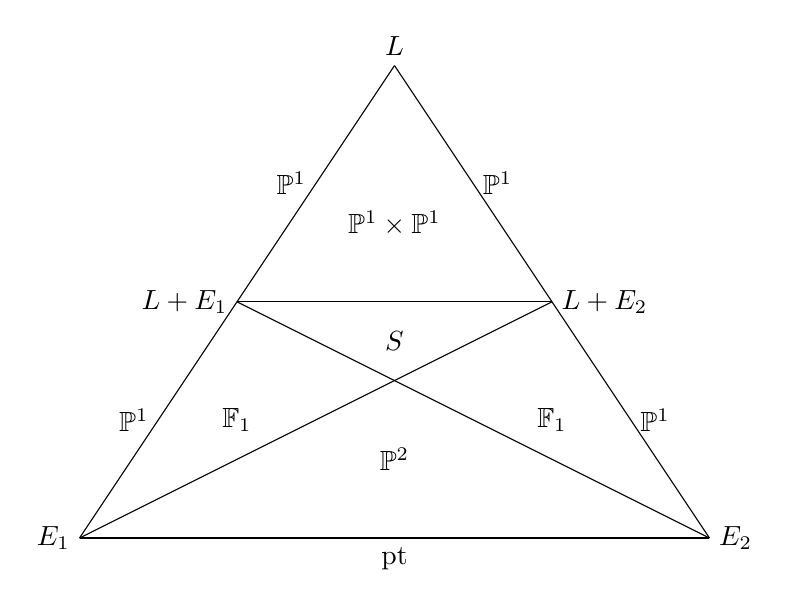
\begin{tikzpicture}
  \draw (-4,0)node[left]{$ E_1 $}--(0,0)node[below]{pt}--(4,0)node[right]{$ E_2 $};
  \draw(-4,0)--(-3,1.5)node[left]{$ \mathbb{P}^1 $}--(-2,3)node[left]{$ L+E_1 $}--(-1,4.5)node[left]{$ \mathbb{P}^1 $}--(0,6)node[above]{$ L $};
  \draw(4,0)--(3,1.5)node[right]{$ \mathbb{P}^1 $}--(2,3)node[right]{$ L+E_2 $}--(1,4.5)node[right]{$ \mathbb{P}^1 $}--(0,6);
  \draw (-2,3)--(4,0);
  \draw (2,3)--(-4,0);
  \draw (-2,3)--(2,3);
  \draw (0,2.5)node{$ S $};
  \draw (2,1.5)node{$ \mathbb{F}_1 $};
  \draw (-2,1.5)node{$ \mathbb{F}_1 $};
  \draw (0,4)node{$ \mathbb{P}^1\times \mathbb{P}^1 $};
  \draw (0,1)node{$ \mathbb{P}^2 $};
\end{tikzpicture}

\subsection{Decompose into links}
We need a special resolution $W$ and an   affine subspace $V \subset \operatorname{WDiv}(W)$ such that we can find two Mori fibre spaces $X/S$ and $Y/T$ and vertexs connecting them. The following  lemma shows the desired affine subspace exits. 
\begin{lem}\label{keylemma}
  Let $ \phi:X\to S $ and $ \psi :Y\to T  $ be two MMP related Mori fibre space corresponding to two klt projective varieties $ (X,B_X) $ and $ (Y,B_Y) $. Then we may find a smooth projective variety $ W $, two biratinal morphism $ f:W\to X $ and $ g:W\to Y $, a klt pair $ (W,B_{W}) $, an ample $ \mathbb{Q} $-divisor $ A $ on $ W $ and a two dimensional rational affine subspace $ V $ of $ \mathrm{WDiv}_\mathbb{R}(W) $ such that 
  \begin{enumerate}[1)]
    \item If $ D\in \mathcal{L}_A(V) $ then $ D-B_W $ is ample;
    \item $ \mathcal{A}_{A,\phi\circ f} $ and $ \mathcal{A}_{A,\psi\circ g} $ are not contained in the boundary of $ \mathcal{L}_A(V) $;
    \item $ V $ satisfy \ref{finiteamplemodel};
    \item $ \mathcal{C}_{A,f} $ and $ \mathcal{C}_{A,g} $ are two dimensional;
    \item $ \mathcal{C}_{A,\phi\circ f} $ and $ \mathcal{C}_{A,\psi\circ g} $ are one dimensional.
  \end{enumerate}
\end{lem}
\begin{proof}

  By assumption there is a $\mathbb{Q}$-factorial klt pair $(W,B_{W})$ such that $f:W\dashrightarrow X$ and $g:W \dashrightarrow Y$are both outcomes of $(K_{W}+B_{W})$-MMP. Let $p':W'\to W$ be any log resolution such that resolves the indeterminacy of $f$ and $g$, then we may write
  \[
    K_{W'}+B_{W'}=p'^*(K_{W}+B_{W})+E'
  \]
where $E'\geqslant 0$ and $B_{W'}\geqslant 0$ have no common components, and $E'$ is exceptional and $p'_*B_{W'}=B_{W}$. Pick a divisor $-F$ which is ample over $W$ with support equal to the full exceptional locus such that $K_{W'}+B_{W'}+F$ is klt. As $p'$ is $(K_{W'}
B_{W'}+F)$-negative and $(K_{W}+B_{W})$ is klt and $W$ is $\mathbb{Q}$-factorial, the $(K_{W'}+B_{W'}+F)$-MMP over $W$ terminates with the pair $(W,B_{W})$. Replacing $(W,B_{W})$ by $(W',B_{W'} +F)$ we may assume that $(W,B_{W})$ is log smooth and $f,g$ are morphisms.

Pick general ample $\mathbb{Q}$-divisors $A, H_{1},H_{2},\ldots ,H_{k}$ on $W$ such that $H_{1},\ldots , H_{k}$ generate te Neron-Seberi group of $W$. Let 
\[
  H=A+H_{1}+\ldots H_{k}
\]
Pick sufficiently ample divisor $A_{S}$ on $S$ and $A_{T}$ on $T$ such that
\[
-(K_{X}+B_{X})+\phi^*A_{S} \text{ and } -(K_{Y}+B_{Y})\psi^*A_{T}
\]
are both ample. Pick a rational number $0<\delta<1$ such that 
\[
  -(K_{X}+B_{X}+\delta f_*H)+\phi^*A_{S} \text{ and } -(K_{Y}+B_{Y}+\delta g_*H)+\psi^*A_{T}
\]
are both ample and $(K_{W}+B_{W}+\delta H)$ is both  $f$ and  $g$ negative. Replacing $H$ by $\delta H$ we may assume that $\delta=1$. Now pick a $\mathbb{Q}$-divisor $B_{0}\leqslant B_{W}$ such that $A+(B_{0}-B_{W}), -(K_{X}+ f_*B_{0}+f_*H)+\phi^*A_{S}$ and $-(K_{Y}+ g_*B_{0}+f_*H)+\psi^*A_{T}$  are all ample and $(K_{W}+B_{0}+H)$ is both  $f$ and  $g$ negative.

Pick general ample $\mathbb{Q}$-divisors $F_{1}\geqslant 0$ and $G_{1}\geqslant 0$  such that
\[
F_{1}\sim_{\mathbb{Q}} -(K_{X}+f_*B_{0}+ f_*H)+\phi^*A_{S} \text{ and } G_{1}\sim_{\mathbb{Q}} -(K_{Y}+g_*B_{0}+ g_*H)+\psi^*A_{T}
\]
and 
\[
  K_{W}+B_{0}+H+F+G
\]
is klt, where $F=f^*F_{1}$ and $G=g^*G_{1}$. 

Let $V_{0}$ be the affine subspace of $\operatorname{WDiv}_{\mathbb{R}}(W)$ which is the tanslate by $B_{0}$ of the vector subspace  spaned by $H_{1},\ldots , H_{k},F,G$. Supppose that $D=A+B \in \mathcal{L}_{A}(V_{0})$. Then 
\[
  D-B_W=(A+B_{0}-B_{W})+(B-B_{0})
\]
is ample, as $B-B_{0}$ is nef by definition of $V_{0}$. Note the 
\[
  B_{0}+F+H \in \mathcal{A}_{A,\phi\circ f}(V_{0}), B_{0}+G+H \in \mathcal{A}_{\psi \circ g}(V_{0})
\]
and $f$, respectively $g$, is a weak log canonical model of $K_{W}+B_{0}+F+H$, respectively $K_{W}+B_{0}+G+H$. Thus theorem \ref{finiteamplemodel} implies that $V_{0}$ satisfies (1-4) of \ref{finiteamplemodel}.

Since $H_{1},\ldots ,H_{k}$ generated the Neron-Severi group of $W$ we may find constants $h_{1},\ldots ,h_{k}$ such that $G \equiv \sum^{k}_{i=1} h_{i}H_{i}$. Then there is $0< \delta\ll 1$ such that  $B_{0}+F+\delta G+H- \delta(\sum_{i=1}^{k} h_{i}H_{i}) \in \mathcal{L}_{A}(V_{0})$ and
\[
  B_{0}+F+\delta G+H-\delta (\sum_i^k h_{i}H_{i}) \equiv B_{0}+F+H
.\]
Thus $\mathcal{A}_{A,\phi\circ f}$ is not contained in the boundary of $\mathcal{L}_{A}(V_{0})$. Similarly $\mathcal{A}_{A,\psi\circ g}$ is not contained in the boundary of $\mathcal{L}_{A}(V_{0})$. In particular $\mathcal{A}_{A,\phi\circ f}$ and   $\mathcal{A}_{A,\psi\circ g}$ span affine hyperplanes of $V_{0}$, since $\rho(X)=\rho(Y)=1$.

Let $V_{1}$ be the tranlate by $B_{0}$ of two dimensional bector space spaned by $F+H-A$ and $F+G-A$. Let $V$ be a small general pertubation of $V_{1}$, which is defined over rationals. This is the affine subspace we need.
\end{proof}
Then we can prove the main theorem
\begin{proof}[Proof of the main theorem]
Let $(W,B_{W}),A $ and $V$ as in the lemma \ref{keylemma}.  Pick $ D_{0} \in \mathcal{A}_{A,\phi\circ f} $  and $ D_1\in \mathcal{C}_{A,g} $ belonging to the interior of $ \mathcal{L}_A(V) $. As $ V $ is two dimensional, removing $ D_0 $ and $ D_1 $ divides the boundary of $ \mathcal{E}_A(V) $ into two parts. The part which consists entirely of divisors which are not big is contained in the interior of $ \mathcal{L}_A(V) $. Consider tracing this boundary from $ D_0 $ to $ D_1 $. Then there are finitely many $ 2\leqslant i\leqslant N $ points $ D_i $ which are contained in more than two polytopes $ \mathcal{C}_{A,f_i}(V) $. By lemma \ref{constructlink},  each point $ D_i $ gives a Sarkisov link. And the birational map $X \dashrightarrow Y$ is composition of such links.
\end{proof}


\section{Applications}




\begin{enumerate}[(A)]
  \item\label{a} \textbf{If $ \lambda\leqslant\mu $ and $ K_X+B+\frac{1}{\mu}H $ is not nef:} Suppose $ f $ is the contraction with respect to a $ (K_X+B) $-negative extremal ray $ R= \overline{\operatorname{ NE }}(X/S) $, then $ (K_X+B+\frac{1}{\mu}H).R=0 $ by definition of $ \mu $. There is an extremal ray $ P \subset \overline{\operatorname{ NE }}(X) $ such that $ (K_X+B+\frac{1}{\mu}H).P<0 $ and $ F:=P+R $ is an extremal face  (Check \cite[5.4.2]{cortiFactoringBirationalMaps} for details). Take  $ 0<t\ll 1 $ such that $ (K_X+B+(\frac{1}{\mu}-t)H).P<0 $, then $  (K_X+B+(\frac{1}{\mu}-t)H).R<0 $ since $H$ is $f$-ample, and $ F $ is a $  (K_X+B+(\frac{1}{\mu}-t)H) $-negative extremal face. Since $ (X,B+(\frac{1}{\mu}-t)H) $ is klt, there is  a contraction $ g:X\to T $ with respect  to $ F $ factorizing through $ f:X\to S $. Since  $ (X,B+\frac{1}{\mu}H) $ is klt, and $ \rho(X/T)=2 $,  we can  run $ (K_X+B+\frac{1}{\mu}H) $-MMP on $ X  $ with scaling of some ample divisor $C$.  Since $ B+\frac{1}{\mu}H $ is relatively big,  the MMP terminates. There are following cases: 
  \begin{enumerate}[1)]
    \item\label{a1} 
\begin{multicols}{2}       % 分两栏 若花括号中为3则是分三列
After finitely many flips $ X\dashrightarrow Z $, first non-flip contraction is a divisorial contraction $ p:Z\to X_1 $, and then followed by a Mori fibre space $(X_{1},B_{1}+\frac{1}{\mu}H_{1} )\to S_{1}$. Then  $S_{1} \cong T$ and this is a link of type III.     

      \[ \xymatrix{
      X\ar[d]_f\ar@{.>}[r]^{flips}&Z\ar[rd]^{p}&\\
      S\ar[dr]&&X_1\ar[d]^{f_1}\\
      &T&S_1\ar[l]_\sim}\]
\end{multicols}
After finitely many flips $ X\dashrightarrow Z $, first non-flip contraction is a divisorial contraction $ p:Z\to X_1 $, and then followed by a Mori fibre space $(X_{1},B_{1}+\frac{1}{\mu}H_{1} )\to S_{1}$. 
    Then  $S_{1} \cong T$ and this is a link of type III.     
      \[ \xymatrix{
      X\ar[d]_f\ar@{.>}[r]^{flips}&Z\ar[rd]^{p}&\\
      S\ar[dr]&&X_1\ar[d]^{f_1}\\
      &T&S_1\ar[l]_\sim}\]
    \item\label{a2}
      \begin{multicols}{2}
      After finitely many flips $ X\dashrightarrow X_1 $, first non-flip contraction is a Mori fibre space $ f_1:X_1\to S_{1} $. This is a link of type IV.  
   \begin{tikzcd} 
     X\ar[d,swap,"f"]\ar[rr,dashrightarrow,"\phi_{1}"]&&X_1\ar[d,"f_1"]\\
      S\ar[dr]&&S_1\ar[dl]\\
      &T &
    \end{tikzcd}
      \end{multicols}


    \item \label{a3}
      \begin{multicols}{2}
      If after finitely many flips $ X\dashrightarrow Z $, first non-flip contraction is a divisorial contraction $ p:Z\to X_1$ with 
    \[ K_Z+B_Z+\frac{1}{\mu}H_Z=p^*(K_{X_1}+B_1+\frac{1}{\mu}H_1)+eE \]
    where $ e>0 $ and  $E=\operatorname{Exc}\,p$ and  $g_{1}: (X_1,B_1+\frac{1}{\mu}H_1) \to T$ is a log minimal model of $(X,B+\frac{1}{\mu}H)$ over $T$ . In fact the only ray of $ \overline{\operatorname{NE}}(X_1/T) $ is $ (K_{X_1}+B_1+\frac{1}{\mu}H_1) $-trivial and hence is $ (K_{X_1}+B_1) $-negative, therefore $ (X_1,B_1)/T $ is a log Mori fibre space. Take $ S_1=T $, then this is a link of type III:
    \[ \xymatrix{
      X\ar[d]_f\ar@{.>}[r]&Z\ar[rd]^{p}&\\
      S\ar[dr]&&X_1\ar[d]^{f_1}\\
      &T&S_1\ar@{=}[l]}\]
\end{multicols}
      If after finitely many flips $ X\dashrightarrow Z $, first non-flip contraction is a divisorial contraction $ p:Z\to X_1$ with 
    \[ K_Z+B_Z+\frac{1}{\mu}H_Z=p^*(K_{X_1}+B_1+\frac{1}{\mu}H_1)+eE \]
    where $ e>0 $ and  $E=\operatorname{Exc}\,p$ and  $g_{1}: (X_1,B_1+\frac{1}{\mu}H_1) \to T$ is a log minimal model of $(X,B+\frac{1}{\mu}H)$ over $T$ . In fact the only ray of $ \overline{\operatorname{NE}}(X_1/T) $ is $ (K_{X_1}+B_1+\frac{1}{\mu}H_1) $-trivial and hence is $ (K_{X_1}+B_1) $-negative, therefore $ (X_1,B_1)/T $ is a log Mori fibre space. Take $ S_1=T $, then this is a link of type III:
    \[ \xymatrix{
      X\ar[d]_f\ar@{.>}[r]&Z\ar[rd]^{p}&\\
      S\ar[dr]&&X_1\ar[d]^{f_1}\\
      &T&S_1\ar@{=}[l]}\]
  \item \label{a4}After finitely many flips $ X\dashrightarrow X_1 $, MMP ends with log minimal model $ (X_1,B_1+\frac{1}{\mu}H_1)/T $. Then there is a ray of $ \overline{\operatorname{NE}}(X_1/T) $ is $ (K_{X_1}+B_1+\frac{1}{\mu}H_1) $-trivial and $ (K_{X_1}+B_1) $-negative.  Take the contraction $ f_1:X_1\to S_1 $ with respect to $ (K_{X_1}+B_1) $-negative ray $ R=\mathbb{R}_{\geqslant 0}[C] $: 
    \[ \xymatrix{
      X\ar[d]_f\ar@{.>}[rr]&&X_1\ar[d]^{f_1}\\
      S\ar[dr]&&S_1\ar[dl]\\
      &T &}\]
    This is a link of type IV. In fact, $X \dashrightarrow  S_{1}$ is the ample model of $K_{X}+B+\frac{1}{\mu}H$.
  \end{enumerate}

\item\label{b} If $ \lambda>\mu $, then $ (X,B+\frac{1}{\mu}H) $ is not $ \theta $-canonical. Take  an extraction $ p:(Z,B_Z,H_Z)\to (X,B,H) $ as in lemma \ref{thetaextraction}, that is  $ (Z,B_Z) $ is $ \theta $-terminal and $ p^*(K_X+B+\frac{1}{\lambda}H)=K_Z+B_Z+\frac{1}{\lambda}H_Z $ where $ B_Z=\sum\theta(E_\nu)E_\nu $ and $ E=\mathrm{Exc}\,p $ is a prime divisor on $ Z $.  Let $ H_Z=p^{-1}_*H $ a strict transform of a general member $ H' $ of $ \mathcal{H}' $. Then we run $ (K_Z+B_Z+\frac{1}{\lambda}H_Z) $-MMP on $ Z $ over $ S $ with scaling of some ample divisor $C$. Since $Z$ is covered by $ (K_Z+B_Z+\frac{1}{\lambda}H_Z) $-negative curves, $ (K_Z+B_Z+\frac{1}{\lambda}H_Z) $ is not relatively pseudo-effective, hence this always ends with a Mori fibre space by theorem \ref{notpseudoeffmfs}. There are two cases:
  \begin{enumerate}[1)]
    \item \label{b1}After finitely many flips $ Z\dashrightarrow Z' $, first non flip contraction is a divisorial contraction $ q:Z'\to X_1 $. Since $ \rho(X_1/S)=1 $, there is no further flips or divisorial contraction, thus must be followed by a fibering contraction $ f_1:X_1\to Y $ with $ Y\xrightarrow{\sim}S $. Since $ (K_{X_1}+B_1+\frac{1}{\lambda}H_1) $ is $ f_1 $-negative, and $ H_1 $ is $ f_1 $- ample, $ (K_{X_1}+B_1) $ is $ f_1 $-negative, and $ (X_1,B_1)/Y $ is a log Mori fibre space.  Let $ S_1=Y $ and this is a link of type II.
    \[ \xymatrix{
      &Z\ar[ld]_p\ar@{.>}[r]&Z'\ar[dr]^{q}&\\
      X\ar[d]_{f}\ar@{.>}[rrr]^{\psi_1}&&&X_1\ar[d]^{f_1}\\
      S\ar@{=}[rrr]&&&S_1} \]
    \item\label{b2} If after finitely many flips $ Z\dashrightarrow X_1 $, first non-flip contraction is a fibering contraction $ f_1:X_1\to Y  $. Since $ (K_{X_1}+B_1+\frac{1}{\lambda}H_1) $ is $ f_1 $-negative and $ H_1 $ is $ f_1 $- ample, $ (K_{X_1}+B_1) $ is $ f_1 $-negative, and $ (X_1,B_1)/Y $ is a log Mori fibre space.  Take $ S_1=Y $ and this is a link of type I.
    \[
      \xymatrix{
      &Z\ar[ld]_p\ar@{.>}[r]&X_1\ar[dd]^{f_1}\\
        X\ar[d]_f&&\\
      S &&S_1\ar[ll]}
    \]
  \end{enumerate} 
\end{enumerate}

\bibliographystyle{alpha}
\bibliography{ref}

\end{document}
